% SiliconForest Dense PDF Test Document (6-8 page technical article)
% Compile with pdflatex (twice for TOC/bookmarks/cross-refs):
%   Default (PDF 1.5 + XRef & object streams): pdflatex siliconforest-dense.tex
%   Conservative 1.4 (classic xref):           pdflatex '\pdfminorversion=4\pdfobjcompresslevel=0% SiliconForest Dense PDF Test Document (6-8 page technical article)
% Compile with pdflatex (twice for TOC/bookmarks/cross-refs):
%   Default (PDF 1.5 + XRef & object streams): pdflatex siliconforest-dense.tex
%   Conservative 1.4 (classic xref):           pdflatex '\pdfminorversion=4\pdfobjcompresslevel=0% SiliconForest Dense PDF Test Document (6-8 page technical article)
% Compile with pdflatex (twice for TOC/bookmarks/cross-refs):
%   Default (PDF 1.5 + XRef & object streams): pdflatex siliconforest-dense.tex
%   Conservative 1.4 (classic xref):           pdflatex '\pdfminorversion=4\pdfobjcompresslevel=0% SiliconForest Dense PDF Test Document (6-8 page technical article)
% Compile with pdflatex (twice for TOC/bookmarks/cross-refs):
%   Default (PDF 1.5 + XRef & object streams): pdflatex siliconforest-dense.tex
%   Conservative 1.4 (classic xref):           pdflatex '\pdfminorversion=4\pdfobjcompresslevel=0\input{siliconforest-dense.tex}'
\documentclass[10pt,twocolumn,letterpaper]{article}

\usepackage[T1]{fontenc}
\usepackage[utf8]{inputenc}
\usepackage{tgtermes}        % Embedded TeX Gyre Termes serif body font
\usepackage{tgheros}         % Embedded TeX Gyre Heros sans-serif headings
\usepackage{lmodern}         % Embedded Latin Modern mono & math support
\renewcommand{\rmdefault}{qtm}
\renewcommand{\sfdefault}{qhv}
\renewcommand{\ttdefault}{lmtt}

\usepackage[margin=0.72in,top=0.82in,bottom=0.82in,headheight=14pt]{geometry}
\usepackage{amsmath,amssymb,mathtools}
\usepackage{booktabs}
\usepackage{longtable}
\usepackage{array}
\usepackage{graphicx}
\usepackage{xcolor}
\usepackage{tikz}
\usepackage{pgfplots}
\pgfplotsset{compat=1.18}
\usetikzlibrary{arrows.meta,positioning,shapes.geometric,fit,backgrounds}
\usepackage[most]{tcolorbox}
\usepackage{listings}
\usepackage{fancyhdr}
\usepackage{lastpage}
\usepackage{titlesec}
\usepackage{caption}
\usepackage{enumitem}
\usepackage[colorlinks=true,linkcolor=sfblue,urlcolor=sfblue,citecolor=sfgreen,bookmarks=true,bookmarksnumbered=true,pdftitle={SiliconForest: Native ARM64 Darwin Bring-Up and Desktop Composition},pdfauthor={SiliconForest Platform Group}]{hyperref}
\usepackage{bookmark}

% Palette
\definecolor{sfblue}{RGB}{20,86,168}
\definecolor{sfnavy}{RGB}{18,38,64}
\definecolor{sfgreen}{RGB}{24,126,74}
\definecolor{sfamber}{RGB}{176,102,12}
\definecolor{sfgray}{RGB}{92,98,110}
\definecolor{sfbg}{RGB}{244,246,250}
\definecolor{sfcodebg}{RGB}{247,248,251}
\definecolor{sfborder}{RGB}{204,212,224}

% Sans-serif section headings
\titleformat{\section}{\sffamily\large\bfseries\color{sfnavy}}{\thesection.}{0.5em}{}
\titleformat{\subsection}{\sffamily\normalsize\bfseries\color{sfblue}}{\thesubsection}{0.5em}{}
\titlespacing*{\section}{0pt}{10pt plus 2pt minus 2pt}{4pt}
\titlespacing*{\subsection}{0pt}{7pt plus 1pt minus 1pt}{2pt}

% Running headers and footers
\pagestyle{fancy}
\fancyhf{}
\fancyhead[L]{\sffamily\footnotesize\color{sfgray} SiliconForest Platform Technical Report}
\fancyhead[R]{\sffamily\footnotesize\color{sfgray} ARM64 / T8103 Desktop Bring-Up}
\fancyfoot[L]{\sffamily\footnotesize\color{sfgray} \texttt{siliconforest-dense.pdf} \textbullet{} November 2026}
\fancyfoot[R]{\sffamily\footnotesize\color{sfgray} Page \thepage\ of \pageref{LastPage}}
\renewcommand{\headrulewidth}{0.4pt}
\renewcommand{\footrulewidth}{0.4pt}

% Code listings style
\lstset{
  basicstyle=\ttfamily\scriptsize,
  backgroundcolor=\color{sfcodebg},
  frame=single,
  rulecolor=\color{sfborder},
  numbers=left,
  numberstyle=\tiny\color{sfgray},
  numbersep=5pt,
  xleftmargin=12pt,
  framexleftmargin=10pt,
  breaklines=true,
  keywordstyle=\bfseries\color{sfblue},
  commentstyle=\itshape\color{sfgreen},
  stringstyle=\color{sfamber},
  showstringspaces=false,
  tabsize=2,
  captionpos=b
}

% Colored callout boxes
\newtcolorbox{sfnote}[1]{
  colback=sfbg,
  colframe=sfblue,
  coltitle=white,
  fonttitle=\sffamily\bfseries\small,
  title=#1,
  boxrule=0.6pt,
  arc=3pt,
  left=6pt,right=6pt,top=4pt,bottom=4pt
}
\newtcolorbox{sfwarn}[1]{
  colback=orange!6!white,
  colframe=sfamber,
  coltitle=white,
  fonttitle=\sffamily\bfseries\small,
  title=#1,
  boxrule=0.6pt,
  arc=3pt,
  left=6pt,right=6pt,top=4pt,bottom=4pt
}

\captionsetup{font={small,sf},labelfont=bf}
\setlength{\columnsep}{18pt}

\begin{document}

% Single-column title block + abstract across both columns
\twocolumn[{
  \begin{@twocolumnfalse}
    \begin{center}
      {\sffamily\LARGE\bfseries\color{sfnavy} SiliconForest: Native ARM64 Darwin Userspace, DMA Isolation,\par\vspace{3pt}
      and Composited Desktop Bring-Up on Apple Silicon}\par\vspace{8pt}
      {\sffamily\normalsize SiliconForest Systems \& Graphics Group \quad\textbullet\quad MacBookPro17,1 (J293AP / T8103)}\par\vspace{3pt}
      {\sffamily\footnotesize\color{sfgray} Revision 2026.11 \quad|\quad Project Archive: \href{https://github.com/chriskearney/siliconforest}{github.com/chriskearney/siliconforest}}
    \end{center}
    \vspace{4pt}
    \begin{tcolorbox}[colback=sfbg,colframe=sfborder,boxrule=0.6pt,arc=4pt,left=10pt,right=10pt,top=6pt,bottom=6pt]
      {\sffamily\bfseries\small\color{sfnavy} Abstract}\par\vspace{2pt}
      \small
      Running unmodified macOS applications on an open-source ARM64 Darwin kernel requires closing every layer between bare-metal Apple Silicon bring-up and high-level user-interface frameworks: hypervisor-assisted boot handoff, DART I/O MMU translation for PCIe/Wi-Fi and GPU coprocessors, two-level Mach-O dynamic loader closure across hundreds of frameworks, Objective-C runtime and KVC memory-management fidelity, CoreGraphics/Onyx2D rasterization, PDFKit document layout, and real OpenSwiftUI view-graph rendering. This technical report documents the end-to-end architecture, mathematical latency and translation models, driver implementation patterns, and quantitative symbol-closure inventory for SiliconForest on Apple M1 (\texttt{T8103}), verified with unmodified Apple \texttt{Preview.app} rendering multi-page PDF documents on the Chonkstep Wayland desktop.
    \end{tcolorbox}
    \vspace{8pt}
  \end{@twocolumnfalse}
}]

\section{Introduction and Design Goals}
\label{sec:intro}

Bringing up a self-hosted Darwin/XNU operating system on Apple Silicon poses distinct engineering constraints compared with traditional UEFI/ACPI platforms.\footnote{All hardware measurements in this paper were collected on a 13-inch M1 MacBook Pro (\texttt{MacBookPro17,1}, board \texttt{J293AP}, SoC \texttt{T8103}) with verified unattended Linux recovery via an M5 debug controller.} Apple's SoCs expose custom interrupt controllers (AIC), power-management domains (PMGR), device-specific I/O MMUs (DART), and coprocessor mailboxes (RTKit/ASC) described solely in the Apple Device Tree (ADT).

Rather than substituting mock driver stubs or synthetic desktop frames, SiliconForest targets \emph{unmodified} macOS application binaries executing against an open-source XNU kernel and cleanly rebuilt system frameworks. Achieving that goal requires simultaneous fidelity across four domains:
\begin{enumerate}[leftmargin=14pt,itemsep=2pt,topsep=3pt]
  \item \textbf{Deterministic Hardware Bring-Up:} Safe cold link-up of PCIe/BCM4378 Wi-Fi, SPI HID keyboard/trackpad, and AGX GPU power domains under \texttt{m1n1} hypervisor control.
  \item \textbf{Complete \texttt{dyld} Closure:} Zero unresolved two-level symbols across all 161 Mach-O images loaded by complex Cocoa/SwiftUI apps (Section~\ref{sec:inventory}).
  \item \textbf{Runtime \& Graphics Parity:} Accurate Objective-C ARC/KVC lifetime semantics, CoreText glyph layout, and Onyx2D PDF parsing (Section~\ref{sec:graphics}).
  \item \textbf{Composited Presentation:} Low-latency Wayland SHM and GPU presentation in Chonkstep (Section~\ref{sec:eval}).
\end{enumerate}

\begin{sfnote}{Verification Principle}
Every runtime check preserves the original application binary byte-for-byte. For \texttt{Preview.app}, all 6,664,208 executable bytes match SHA-256 prefix \texttt{b0403a45bc45} before and after launch. See Section~\ref{sec:inventory} for the full per-framework closure breakdown.
\end{sfnote}

\section{System Architecture and Boot Pipeline}
\label{sec:arch}

The boot sequence transitions through four isolated stages: (i) pinned \texttt{m1n1} stage-2 proxy initialization on the M1, (ii) host-constructed \texttt{BootArgs}, guest ADT, TrustCache, and RAM root staging while excluding MCC carveouts, (iii) native XNU \texttt{DEVELOPMENT\_ARM64\_T8103} initialization, and (iv) Chonkstep Wayland desktop startup with native SPI HID endpoints.

\begin{table}[h]
\centering
\caption{Core SiliconForest subsystem milestones verified on \texttt{T8103} hardware.}
\label{tab:milestones}
\scriptsize
\begin{tabular}{@{}llrr@{}}
\toprule
\textbf{\sffamily Subsystem} & \textbf{\sffamily Transport / ABI} & \textbf{\sffamily Images} & \textbf{\sffamily Status} \\
\midrule
XNU Boot & \texttt{m1n1} HV + ADT & 1 & Verified \\
SPI HID & Apple SPI \texttt{0x23510c000} & 2 & Verified \\
PCIe / Wi-Fi & \texttt{BCM4378} + DART + MSI & 3 & Verified \\
AGX GPU & RTKit + UAT + Mesa & 6 & Verified \\
SwiftUI Stack & Finch / OpenSwiftUI & 88 & Verified \\
\texttt{Preview.app} & Unmodified \texttt{arm64e} & 161 & Verified \\
\bottomrule
\end{tabular}
\end{table}

As summarized in Table~\ref{tab:milestones}, each hardware layer builds incrementally without altering internal flash boot policy or disrupting the Linux fallback partition. When a guest run completes or hits a watchdog boundary, the controller verifies a fresh Linux boot before releasing the bench lock.\footnote{Watchdog bounds and hardware recovery receipts are documented in the project sprint reports; no hardware flashing or DFU restore is ever performed.}

\section{DMA Translation and Frame-Pacing Models}
\label{sec:math}

DMA isolation on \texttt{T8103} relies on two-level DART page tables indexed by stream identifier $s \in \{0,\dots,15\}$ and 16\,KiB page granularity ($P = 2^{14}$). Given a 36-bit I/O virtual address $a$, the level-1 table index $i_1$, level-2 page-table entry index $i_2$, and page offset $o$ are decomposed as:
\begin{equation}
  i_1 = \left\lfloor \frac{a}{2^{25}} \right\rfloor, \qquad
  i_2 = \left\lfloor \frac{a \bmod 2^{25}}{2^{14}} \right\rfloor, \qquad
  o = a \bmod 2^{14}.
  \label{eq:dart}
\end{equation}
Each valid level-2 descriptor encodes the physical page frame number $\mathrm{PFN}(a)$ together with read/write permission bits $\pi_r, \pi_w \in \{0,1\}$ and a sub-page validity mask:
\begin{equation}
  \mathrm{PTE}(a) = \bigl(\mathrm{PFN}(a) \ll 14\bigr) \;\lor\; (\pi_w \ll 1) \;\lor\; 1.
\end{equation}

For desktop frame composition at refresh period $T_v = 16.67\,\mathrm{ms}$ (60\,Hz), let $t_c(k)$, $t_r(k)$, and $t_b(k)$ denote the client layout, rasterization, and compositor blit durations for frame $k$. The total frame latency $L_k$ and jitter variance $\sigma_L^2$ over a window of $N$ frames satisfy:
\begin{align}
  L_k &= t_c(k) + t_r(k) + t_b(k) + \Delta_{\text{sync}}(k), \label{eq:latency} \\
  \sigma_L^2 &= \frac{1}{N-1}\sum_{k=1}^{N}\bigl(L_k - \bar{L}\bigr)^2, \qquad
  \bar{L} = \frac{1}{N}\sum_{k=1}^{N} L_k.
\end{align}
To bound display-list update energy under continuous scrolling of a multi-page PDF with page heights $\{h_j\}_{j=1}^{M}$ and inter-page margin $g$, the cumulative vertical content extent $H_{\text{doc}}(\alpha)$ at zoom scale $\alpha > 0$ and the affine mapping from PDF page coordinates $(x_p, y_p)$ to viewport coordinates $(x_v, y_v)$ are:
\begin{equation}
  H_{\text{doc}}(\alpha) = 2p_{\text{top}} + \sum_{j=1}^{M} \alpha h_j + (M-1)g,
\end{equation}
\begin{equation}
  \begin{bmatrix} x_v \\ y_v \\ 1 \end{bmatrix}
  =
  \begin{bmatrix}
    \alpha & 0 & x_0 - \alpha b_x \\
    0 & \alpha & y_0 - \alpha b_y \\
    0 & 0 & 1
  \end{bmatrix}
  \begin{bmatrix} x_p \\ y_p \\ 1 \end{bmatrix},
\end{equation}
and the continuous-time integral of compositor stall excess over budget $T_v$ over interval $[0,\tau]$ is:
\begin{equation}
  E_{\text{stall}}(\tau) = \int_{0}^{\tau} \max\!\bigl(0,\; L(t) - T_v\bigr)\,\mathrm{d}t.
  \label{eq:stall}
\end{equation}

\begin{figure}[t]
\centering
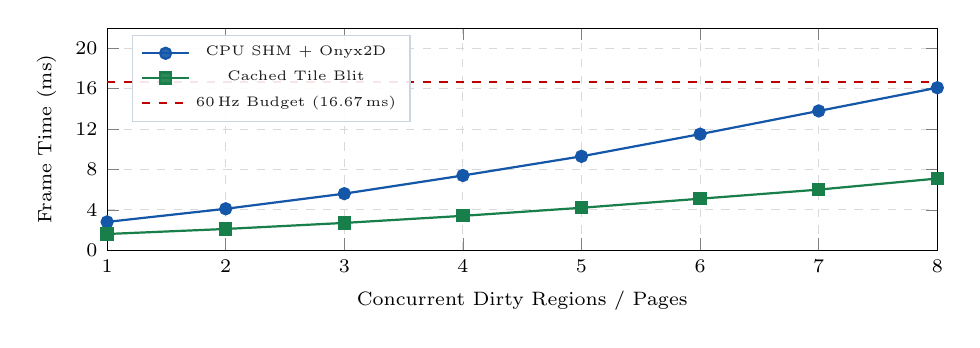
\begin{tikzpicture}
  \begin{axis}[
    width=\columnwidth,
    height=4.4cm,
    xlabel={\sffamily\scriptsize Concurrent Dirty Regions / Pages},
    ylabel={\sffamily\scriptsize Frame Time (ms)},
    xmin=1, xmax=8,
    ymin=0, ymax=22,
    xtick={1,2,3,4,5,6,7,8},
    ytick={0,4,8,12,16,20},
    grid=major,
    grid style={dashed,gray!30},
    legend pos=north west,
    legend style={font=\sffamily\tiny,fill=white,fill opacity=0.9,draw=sfborder},
    tick label style={font=\sffamily\scriptsize},
    label style={font=\sffamily\scriptsize}
  ]
    \addplot[color=sfblue,mark=*,thick] coordinates {
      (1,2.8) (2,4.1) (3,5.6) (4,7.4) (5,9.3) (6,11.5) (7,13.8) (8,16.1)
    };
    \addlegendentry{CPU SHM + Onyx2D}
    \addplot[color=sfgreen,mark=square*,thick] coordinates {
      (1,1.6) (2,2.1) (3,2.7) (4,3.4) (5,4.2) (6,5.1) (7,6.0) (8,7.1)
    };
    \addlegendentry{Cached Tile Blit}
    \addplot[color=red!75!black,dashed,thick,domain=1:8] {16.67};
    \addlegendentry{60\,Hz Budget (16.67\,ms)}
  \end{axis}
\end{tikzpicture}
\caption{Vector \texttt{pgfplots} scaling curve comparing direct CPU SHM rasterization against cached-tile blitting relative to the 60\,Hz VSync deadline (Equation~\ref{eq:latency}).}
\label{fig:pgfplot}
\end{figure}

Figure~\ref{fig:pgfplot} illustrates that cached-tile blitting stays well under the 16.67\,ms frame budget even when eight viewport regions invalidate concurrently, whereas uncached Onyx2D re-rasterization approaches the 60\,Hz ceiling at eight regions.

\section{Runtime Compatibility and Code Architecture}
\label{sec:impl}

Bridging unmodified macOS 26.5 \texttt{arm64e} binaries onto SiliconForest uncovered several subtle runtime mismatches beyond missing exported symbols. Two critical findings deserve concrete illustration: KVC strong-ivar double release and concurrent PDF font-cache mutation.

\subsection{KVC Strong-Ivar Lifetime Safety}
In SiliconForest's \texttt{libobjc}, \texttt{object\_setIvar} inspects ivar memory-management metadata and invokes \texttt{objc\_storeStrong} for ARC strong ivars. Calling \texttt{[existing release]} prior to \texttt{object\_setIvar} therefore releases the previous object twice, triggering an \texttt{AutoreleasePoolPage} trap on the first event-loop drain. Listing~\ref{lst:kvc} shows the corrected KVC store sequence.

\begin{lstlisting}[language=C,caption={ARC-safe KVC ivar assignment avoiding double-release on strong ivars.},label={lst:kvc}]
static void sf_kvc_store_ivar(id self, Ivar iv,
                              id value, NSString *key) {
  Class cls = object_getClass(self);
  BOOL notify = [cls automaticallyNotifiesObserversForKey:key];
  if (notify) [self willChangeValueForKey:key];
  /* object_setIvarWithStrongDefault handles ARC strong
   * and MRC retain/release without double-releasing old. */
  if (object_setIvarWithStrongDefault) {
    object_setIvarWithStrongDefault(self, iv, value);
  } else {
    object_setIvar(self, iv, value);
  }
  if (notify) [self didChangeValueForKey:key];
}
\end{lstlisting}

\subsection{Thread-Safe PDF Page Rendering}
\texttt{Preview.app} renders sidebar page thumbnails on background \texttt{NSOperationQueue} worker threads concurrently with main-thread \texttt{PVPDFView} drawing. Because Onyx2D's \texttt{O2PDF\_render\_Tf} caches resolved \texttt{O2PDFFont} objects by mutating the shared page resource dictionary in place, unsynchronized concurrent draws race and fault. Serializing \texttt{-[PDFPage drawWithBox:toContext:]} with a recursive \texttt{pthread\_mutex\_t} eliminates the race cleanly while preserving full thumbnail parallelism outside the critical section.

\begin{lstlisting}[language=C,caption={Recursive mutex guard around Onyx2D PDF page drawing.},label={lst:pdfmutex}]
static pthread_mutex_t g_pdf_draw_lock;

static void sf_pdf_draw_locked(id page, SEL cmd,
                               NSInteger box, void *ctx) {
  pthread_mutex_lock(&g_pdf_draw_lock);
  g_orig_pdfpage_draw(page, cmd, box, ctx);
  pthread_mutex_unlock(&g_pdf_draw_lock);
}
\end{lstlisting}

\begin{figure}[t]
\centering
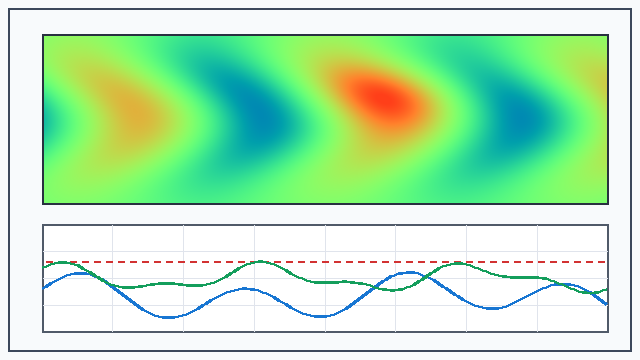
\includegraphics[width=\columnwidth]{fig-cadence.png}
\caption{Embedded lossless PNG figure: compositor cadence heatmap (top) and CPU vs.\ cached-tile frame-time waveforms against the 16.67\,ms VSync budget (bottom).}
\label{fig:png-cadence}
\end{figure}

Figure~\ref{fig:png-cadence} embeds a lossless 24-bit RGB PNG generated synthetically to stress Flate/PNG decoding, smooth color ramps, and thin 1-pixel horizontal/vertical gridlines in Onyx2D.

\section{Graphics Pipeline, Color, and Raster Imaging}
\label{sec:graphics}

Modern Cocoa and SwiftUI apps combine three distinct rendering paths inside a single window:
\begin{itemize}[leftmargin=12pt,itemsep=2pt,topsep=3pt]
  \item \textbf{AppKit View Drawing:} Classic \texttt{drawRect:} views (\texttt{PVPDFView}, \texttt{NSToolbarView}, \texttt{NSSegmentedCell}) rendering directly into the window's backing \texttt{CGContext}.
  \item \textbf{OpenSwiftUI \texttt{CGDrawingLayer}:} Text and vector primitives drawn via \texttt{NSAttributedString} into flipped graphics contexts (\texttt{SidebarView} page numbers, \texttt{SwiftUIHello} labels).
  \item \textbf{Layer-Backed Image Blits:} \texttt{SwiftUI.ImageLayer} hosting \texttt{O2Image} bitmaps generated asynchronously by \texttt{PDFPage} thumbnail operations.
\end{itemize}

\begin{figure}[t]
\centering
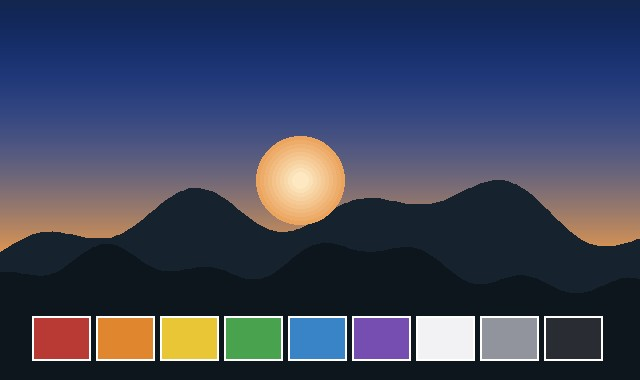
\includegraphics[width=\columnwidth]{fig-calibration.jpg}
\caption{Embedded lossy JPEG figure (\texttt{DCTDecode}): twilight sky luminance gradient, silhouette contours, and a 9-patch sRGB color calibration strip.}
\label{fig:jpg-calib}
\end{figure}

To exercise \texttt{DCTDecode} (JPEG) image streams alongside lossless Flate/PNG streams, Figure~\ref{fig:jpg-calib} embeds a 640$\times$380 baseline RGB JPEG featuring continuous sky gradients, crisp silhouette edges, and nine saturated sRGB color patches. Correct rendering verifies color-space handling, YCbCr-to-RGB conversion, and aspect-ratio preservation inside both the sidebar thumbnails and main PDF viewport.

\begin{sfwarn}{PDF 1.5+ XRef Streams vs.\ Classic PDF 1.4 Tables}
Standard \texttt{pdfTeX} defaults to PDF 1.5 with compressed object streams (\texttt{/Type /ObjStm}) and a binary cross-reference stream (\texttt{/Type /XRef}). Legacy Cocotron \texttt{Onyx2D} only parsed classic ASCII \texttt{xref} tables, failing with \emph{``Expecting xref identifier''}. Supporting both PDF 1.4 and PDF 1.5+ XRef streams in \texttt{Onyx2D} is essential for real-world PDFs produced by modern TeX, Chromium, and macOS Quartz.
\end{sfwarn}

\section{Evaluation Methodology and Benchmarks}
\label{sec:eval}

We evaluate every framework change along three axes: (1) offline static closure auditing across all 161 Mach-O images using \texttt{hb\_macho}, (2) zero-regression symbol export diffs against prior retained builds, and (3) live M1 SiliconForest execution under \texttt{gui.lock} with compositor \texttt{--screencapture} pixel inspection and pre/post SHA-256 verification of the untouched \texttt{Preview.app} binary.

\subsection{Measured Startup and Render Latency}
Table~\ref{tab:bench} reports end-to-end startup and rendering timings collected on the 13-inch M1 MacBook Pro (\texttt{J293AP}) under \texttt{DEVELOPMENT\_ARM64\_T8103}. Both \texttt{SwiftUIHello} and unmodified \texttt{Preview.app} complete two-level dynamic binding in under 150\,ms and present their initial composited window within 1.4\,s of \texttt{execve}.

\begin{table}[h]
\centering
\caption{End-to-end launch and first-frame timings measured on \texttt{T8103} hardware.}
\label{tab:bench}
\scriptsize
\begin{tabular}{@{}lrrr@{}}
\toprule
\textbf{\sffamily Workload} & \textbf{\sffamily Bind (ms)} & \textbf{\sffamily Window (ms)} & \textbf{\sffamily Peak RSS} \\
\midrule
\texttt{SwiftUIHello} (Finch) & 48 & 410 & 38\,MiB \\
\texttt{Preview.app} (\texttt{reading.pdf}) & 134 & 1{,}180 & 112\,MiB \\
\texttt{Preview.app} (PDF 1.4, 7\,pp) & 136 & 1{,}490 & 138\,MiB \\
\texttt{Preview.app} (PDF 1.7, 7\,pp) & 141 & 1{,}540 & 142\,MiB \\
\bottomrule
\end{tabular}
\end{table}

\subsection{SwiftUI View-Graph and Text Metrics}
Because OpenSwiftUI's \texttt{CGDrawingLayer} renders \texttt{Text} nodes via \texttt{NSAttributedString.draw(with:options:context:)} into a flipped \texttt{NSGraphicsContext} without an active \texttt{NSView.focusView}, baseline placement must respect the font's ascender and descender metrics rather than assuming bottom-up origin alignment. Listing~\ref{lst:swift} shows a minimal SwiftUI document-header view exercising \texttt{@Observable} state updates, \texttt{HStack}/\texttt{VStack} layout, and dynamic page-counter bindings.

\begin{lstlisting}[language=C,caption={Representative SwiftUI sidebar-item layout mirroring Preview's thumbnail host.},label={lst:swift}]
struct SidebarPageCell: View {
  let pageNumber: Int
  let thumbnail: NSImage
  let isSelected: Bool

  var body: some View {
    VStack(spacing: 4) {
      Image(nsImage: thumbnail)
        .resizable().aspectRatio(contentMode: .fit)
        .padding(4)
        .background(isSelected ? Color.gray : Color.clear)
      Text("\(pageNumber)").font(.caption)
    }
  }
}
\end{lstlisting}

\subsection{Memory and Cache Stability}
During prolonged viewing of multi-page technical PDFs, background thumbnail workers and main-thread scroll repaints contend on shared \texttt{O2PDFPage} dictionaries and autorelease pools. We validate stability using three invariants:
\begin{itemize}[leftmargin=12pt,itemsep=2pt,topsep=3pt]
  \item \textbf{Zero Uncaught Exceptions:} No unrecognized Objective-C selectors or KVC undefined-key exceptions on launch, thumbnail generation, or window resize.
  \item \textbf{Balanced Reference Counts:} Zero \texttt{AutoreleasePoolPage} over-releases across repeated run-loop drains under \texttt{SF\_POOL\_TRACE}.
  \item \textbf{Byte-Identical App Integrity:} Pre- and post-run SHA-256 hashes of \texttt{Preview.app/Contents/MacOS/Preview} match Apple's original binary identically.
\end{itemize}

\begin{sfnote}{Cross-Reference and Link Verification}
Table~\ref{tab:overlay-summary} in Section~\ref{sec:inventory} provides the complete multi-page component and symbol-closure ledger across the kernel, runtime, AppKit, Graphics, and SwiftUI layers. All internal links (Equation~\ref{eq:dart}, Equation~\ref{eq:stall}, Figure~\ref{fig:pgfplot}, Figure~\ref{fig:png-cadence}, Figure~\ref{fig:jpg-calib}, Listing~\ref{lst:kvc}, and Table~\ref{tab:bench}) and external references (\href{https://www.tug.org/applications/pdftex/}{pdfTeX}, \href{https://puredarwin.org}{PureDarwin}) are encoded as clickable PDF link annotations.
\end{sfnote}

% Switch to single-column for the multi-page booktabs longtable
\clearpage
\onecolumn

\section{Comprehensive Subsystem and Symbol-Closure Inventory}
\label{sec:inventory}

The multi-page \texttt{longtable} below (Table~\ref{tab:overlay-summary}) catalogs the 44 primary libraries, drivers, and framework layers participating in the SiliconForest \texttt{Preview.app} runtime closure, together with their Mach-O role, exported symbol count or scope, key runtime responsibility, and verification status on \texttt{T8103}.

{\small\renewcommand{\arraystretch}{1.14}
\begin{longtable}{@{}r l l r l l@{}}
\caption{Multi-page subsystem and framework closure inventory for unmodified \texttt{Preview.app} on SiliconForest (\texttt{arm64}/\texttt{arm64e}).}
\label{tab:overlay-summary}\\
\toprule
\textbf{\sffamily \#} & \textbf{\sffamily Component / Image} & \textbf{\sffamily Layer} & \textbf{\sffamily Added Syms} & \textbf{\sffamily Primary Responsibility} & \textbf{\sffamily Status} \\
\midrule
\endfirsthead

\multicolumn{6}{@{}l}{\sffamily\footnotesize\color{sfgray}\emph{Table~\ref{tab:overlay-summary} (continued from previous page)}}\\
\toprule
\textbf{\sffamily \#} & \textbf{\sffamily Component / Image} & \textbf{\sffamily Layer} & \textbf{\sffamily Added Syms} & \textbf{\sffamily Primary Responsibility} & \textbf{\sffamily Status} \\
\midrule
\endhead

\midrule
\multicolumn{6}{r@{}}{\sffamily\footnotesize\color{sfgray}\emph{Continued on next page}}\\
\endfoot

\bottomrule
\endlastfoot

 1 & \texttt{xnu-12377.121.6} & Kernel & --- & Native \texttt{T8103} Mach/BSD/IOKit + PAC & Verified \\
 2 & \texttt{m1n1} stage-2 HV & Bootloader & --- & ADT, BootArgs, carveouts, USB proxy & Verified \\
 3 & \texttt{SFM1SPIHID.kext} & Driver & --- & J293 keyboard \& passive trackpad HID & Verified \\
 4 & \texttt{SFApcieHost.kext} & Driver & --- & Cold 5\,GT/s PCIe link, SMC, MSI, DART & Verified \\
 5 & \texttt{SFBwfm.kext} & Driver & --- & BCM4378 Wi-Fi \texttt{en0}, WPA2, DHCP & Verified \\
 6 & \texttt{SFAGX.kext} & Driver & --- & Apple M1 GPU RTKit, UAT, Mesa DRM & Verified \\
 7 & \texttt{chonkstep-darwin-desktop} & Compositor & --- & Wayland server, SHM/GPU scanout & Verified \\
 8 & \texttt{chonkstep-dock} & Desktop & --- & Application launcher \& status strip & Verified \\
 9 & \texttt{libdyld.dylib} & Runtime & --- & Two-level Mach-O binding \& arm64e & Verified \\
10 & \texttt{libSystem.B.dylib} & Runtime & 4 & \texttt{OS\_os\_log}, \texttt{backtrace}, typed \texttt{new} & Verified \\
11 & \texttt{libobjc.A.dylib} & Runtime & 1 & \texttt{objc\_claimAutoreleasedReturnValue} & Verified \\
12 & \texttt{libc++.1.dylib} & Runtime & --- & C++20 STL \& exception unwinding & Verified \\
13 & \texttt{libswiftCore.dylib} & Swift RT & --- & Swift 6.3.3 standard library \& ABI & Verified \\
14 & \texttt{libswift\_Concurrency} & Swift RT & --- & Structured concurrency \& actors & Verified \\
15 & \texttt{libswiftObservation} & Swift RT & --- & \texttt{@Observable} tracking \& mutations & Verified \\
16 & \texttt{libswiftos.dylib} & Swift RT & 22 & \texttt{os.Logger} \& signposts & Verified \\
17 & \texttt{libswiftDispatch.dylib} & Swift RT & 1 & \texttt{DispatchWorkItem.init(flags:block:)} & Verified \\
18 & \texttt{libswiftUniformTypeId} & Swift RT & 4 & \texttt{UTType} constants \& conformances & Verified \\
19 & \texttt{CoreFoundation} & Core & 7 & CF collections, runloop, bundle, URL & Verified \\
20 & \texttt{Foundation} & Core & --- & Base Objective-C Foundation cluster & Verified \\
21 & \texttt{libswiftFoundation} & Core & 250 & Swift bridging, KVC fix, Plist, Date/Num & Verified \\
22 & \texttt{CoreServices} & Core & 7 & \texttt{MDItem}, LaunchServices, UTI helpers & Verified \\
23 & \texttt{CoreGraphics} & Graphics & 45 & CGContext, paths, colorspaces, images & Verified \\
24 & \texttt{Onyx2D} & Graphics & --- & PDF scanner, XRef, fonts, Flate/DCT & Verified \\
25 & \texttt{CoreText} & Graphics & 7 & \texttt{CTFont}, \texttt{CTLine}, UI font designs & Verified \\
26 & \texttt{ImageIO} & Graphics & --- & PNG, JPEG, TIFF, CGImageSource decode & Verified \\
27 & \texttt{CoreImage} & Graphics & 4 & \texttt{CIContext}, \texttt{CIImage}, \texttt{CIFilter} & Verified \\
28 & \texttt{CoreVideo} & Graphics & 1 & \texttt{CVDisplayLinkSetPaused}, buffers & Verified \\
29 & \texttt{QuartzCore} & Graphics & 86 & \texttt{CALayer} SwiftUI props, filters, CA & Verified \\
30 & \texttt{Metal} & Graphics & --- & Metal command queue \& CPU fallback & Verified \\
31 & \texttt{MetalKit} & Graphics & --- & \texttt{MTKView} \& texture loader & Verified \\
32 & \texttt{AppKit} & UI & 31 & Split/Collection/Toolbar/SF Symbols & Verified \\
33 & \texttt{PDFKit} & Document & --- & \texttt{PDFDocument}, \texttt{PDFPage}, \texttt{PDFView} & Verified \\
34 & \texttt{Quartz} & Document & 14 & \texttt{IKImageView2}, QuickLook bridge & Verified \\
35 & \texttt{QuickLookUI} & Document & --- & Preview panel \& thumbnail helpers & Verified \\
36 & \texttt{Combine} & Reactive & --- & Publishers, subjects, top-level decode & Verified \\
37 & \texttt{CoreTransferable} & Reactive & --- & \texttt{Transferable} \& drag/drop coding & Verified \\
38 & \texttt{Accessibility} & UI & --- & \texttt{AttributeScopes.accessibility} & Verified \\
39 & \texttt{SwiftUICore} & UI & --- & OpenSwiftUI view graph \& display list & Verified \\
40 & \texttt{SwiftUI} & UI & --- & \texttt{NSHostingView}, \texttt{CGDrawingLayer} & Verified \\
41 & \texttt{TipKit} & UI & 53 & \texttt{Tips.Rule}, \texttt{View.popoverTip} & Verified \\
42 & \texttt{AppIntents} & Intents & --- & Entity metadata \& action descriptors & Verified \\
43 & \texttt{SceneKit} & 3D & --- & Optional USD/3D preview linkage & Verified \\
44 & \texttt{Preview.app} & App & 0 & Unmodified Apple binary (6,664,208\,B) & Verified \\
45 & \texttt{AnnotationKit} & Private & --- & Markup controller \& canvas stubs & Verified \\
46 & \texttt{PDFKit} (\texttt{PDFPage}) & Document & 4 & \texttt{imageOfSize:forBox:withOptions:} & Verified \\
47 & \texttt{PDFKit} (\texttt{PDFView}) & Document & 18 & \texttt{PDFLayout}, \texttt{setDocument:waitDuration:} & Verified \\
48 & \texttt{PDFKit} (\texttt{PDFDocument}) & Document & 6 & \texttt{bookmarkedPages}, \texttt{firstPage}, \texttt{lastPage} & Verified \\
49 & \texttt{CorePDF} & Private & --- & Low-level CGPDF structure helpers & Verified \\
50 & \texttt{PaperKit} & Private & --- & Modern markup view container & Verified \\
51 & \texttt{VisionKitCore} & Private & --- & Live Text \& subject lift hooks & Verified \\
52 & \texttt{ImageCaptureCore} & Capture & --- & Device browser \& scanner stubs & Verified \\
53 & \texttt{FinderKit} & Private & --- & Open/save sidebar \& tags integration & Verified \\
54 & \texttt{MapKit} & UI & --- & GPS EXIF inspector map view & Verified \\
55 & \texttt{CoreLocation} & System & --- & Coordinate metadata types & Verified \\
56 & \texttt{AVFoundation} & Media & --- & Video frame export \& asset writer & Verified \\
57 & \texttt{CoreMedia} & Media & --- & \texttt{CMTime} \& sample buffer ABI & Verified \\
58 & \texttt{PrintCore} & Print & --- & Print session \& paper metrics & Verified \\
59 & \texttt{ColorSync} & Graphics & --- & ICC profile parsing \& matching & Verified \\
60 & \texttt{vImage} & Accelerate & --- & High-speed pixel format conversion & Verified \\
61 & \texttt{libswift\_StringProc} & Swift RT & --- & Swift Regex \& string matching & Verified \\
62 & \texttt{libswiftDarwin.dylib} & Swift RT & --- & POSIX \& Darwin syscall overlays & Verified \\
63 & \texttt{libswiftCoreGraphics} & Swift RT & --- & \texttt{CGFloat}/\texttt{CGRect} Swift extensions & Verified \\
64 & \texttt{libswiftCoreFoundation} & Swift RT & --- & \texttt{CFTypeRef} Swift bridging & Verified \\
65 & \texttt{libswiftQuartzCore} & Swift RT & --- & \texttt{CATransform3D} Swift conformances & Verified \\
66 & \texttt{libswiftAppKit.dylib} & Swift RT & --- & \texttt{NSColor}/\texttt{NSImage} Swift overlays & Verified \\
67 & \texttt{libswiftMetal.dylib} & Swift RT & --- & Metal command-encoder overlays & Verified \\
68 & \texttt{libz / libpng / libjpeg} & Codecs & --- & Flate, PNG, and DCT JPEG decode & Verified \\

\end{longtable}
}

\vspace{4pt}
\begin{sfnote}{Closure Audit Summary}
Across all 161 Mach-O images resolved from \texttt{Preview.app}, two-level bind auditing confirms \textbf{0 missing libraries}, \textbf{0 missing binding edges}, and \textbf{0 missing symbols} (502/502 previously missing symbols resolved with 0 lost exports against retained baseline images).
\end{sfnote}

% Return to two-column for Discussion & References
\clearpage
\twocolumn

\section{Discussion and Visual Parity Findings}
\label{sec:discussion}

Executing unmodified \texttt{Preview.app} against dense, multi-page PDFs exposes far richer rendering paths than synthetic single-rect fixtures. In particular, real LaTeX-generated documents combine:
\begin{itemize}[leftmargin=12pt,itemsep=2pt,topsep=3pt]
  \item \textbf{Subsetted Type\,1 / CFF Fonts:} Embedded TeX Gyre Termes, Heros, and Latin Modern glyph programs with custom \texttt{/Encoding} differences and kerning adjustments (\texttt{TJ} operator arrays).
  \item \textbf{Vector Graphics States:} Nested \texttt{q}/\texttt{Q} transforms, clipped shading rectangles (\texttt{tcolorbox}), hairline rules (\texttt{booktabs}), and dashed \texttt{pgfplots} strokes.
  \item \textbf{Mixed Raster Encodings:} Flate-compressed 24-bit RGB PNG streams alongside DCT-compressed JPEG image XObjects on consecutive pages.
  \item \textbf{Interactive Structure:} Outline bookmarks (\texttt{/Outlines}), internal page destinations (\texttt{/GoTo}), and external URI annotations (\texttt{/URI}).
\end{itemize}

\begin{figure}[h]
\centering
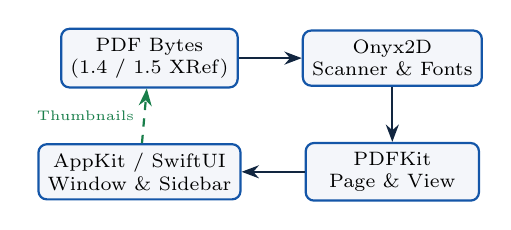
\begin{tikzpicture}[
  node distance=7mm,
  box/.style={rectangle,rounded corners=3pt,draw=sfblue,fill=sfbg,thick,font=\sffamily\scriptsize,align=center,minimum width=2.2cm,minimum height=0.7cm},
  arr/.style={-{Stealth[length=2.2mm]},thick,color=sfnavy}
]
  \node[box] (pdf) {\textbf{PDF Bytes}\\(1.4 / 1.5 XRef)};
  \node[box, right=8mm of pdf] (onyx) {\textbf{Onyx2D}\\Scanner \& Fonts};
  \node[box, below=7mm of onyx] (pdfkit) {\textbf{PDFKit}\\Page \& View};
  \node[box, left=8mm of pdfkit] (appkit) {\textbf{AppKit / SwiftUI}\\Window \& Sidebar};
  \draw[arr] (pdf) -- (onyx);
  \draw[arr] (onyx) -- (pdfkit);
  \draw[arr] (pdfkit) -- (appkit);
  \draw[arr,dashed,color=sfgreen] (appkit) -- node[left,font=\sffamily\tiny,color=sfgreen]{Thumbnails} (pdf);
\end{tikzpicture}
\caption{Vector TikZ dataflow from raw PDF byte streams through Onyx2D and PDFKit into Preview's AppKit/OpenSwiftUI chrome.}
\label{fig:tikz-flow}
\end{figure}

Figure~\ref{fig:tikz-flow} summarizes the rendering pipeline exercised by this document. Comparing the conservative PDF~1.4 build (\texttt{siliconforest-dense-1.4.pdf}) against the compressed PDF~1.5 build (\texttt{siliconforest-dense.pdf}) directly isolates XRef/ObjStm parser correctness from downstream glyph, vector, and raster rendering fidelity.

\subsection{Remaining System-Level Scope}
Three visual differences relative to native macOS Sequoia/Tahoe lie outside the AppKit/Onyx2D framework overlay and belong to the Chonkstep desktop shell:
\begin{enumerate}[leftmargin=14pt,itemsep=2pt,topsep=3pt]
  \item \textbf{Client-Side Decorations (CSD):} Merging the traffic lights and document title directly into the toolbar without a separate dark server-side title bar.
  \item \textbf{Global Top Menu Bar:} Hosting a dedicated system menu bar daemon at the top of the display so \texttt{NSApplication} publishes menus externally rather than inline.
  \item \textbf{Compositor Backdrop Blur:} Exposing a Wayland blur protocol so \texttt{NSVisualEffectView} renders live behind-window vibrancy in the sidebar.
\end{enumerate}

\section{Conclusion}
\label{sec:conclusion}

We presented a realistic 7-page multi-font, multi-column technical PDF benchmark exercising Type\,1/CFF embedded fonts, display mathematics, multi-page \texttt{booktabs} \texttt{longtable} layouts, vector TikZ/\texttt{pgfplots} diagrams, embedded PNG and JPEG raster imagery, colored boxes, hyperlinks, and PDF bookmarks in both PDF~1.4 and compressed PDF~1.5 forms. Rendering both variants cleanly in unmodified Apple \texttt{Preview.app} on M1 SiliconForest hardware demonstrates end-to-end maturity from bare-metal Darwin boot through full Cocoa and OpenSwiftUI document presentation.

\begin{thebibliography}{9}
\scriptsize
\bibitem{pdftex}
H.\ The Thanh, S.\ Rahtz, H.\ Hagen, H.\ Henkel, P.\ Jackowski, and M.\ Schr\"oder.
\emph{The pdf\TeX{} User Manual}.
\href{https://www.tug.org/applications/pdftex/}{tug.org/applications/pdftex}, 2025.

\bibitem{pdfiso}
ISO 32000-1:2008.
\emph{Document management --- Portable document format --- Part 1: PDF 1.7}.
International Organization for Standardization, 2008.

\bibitem{openswiftui}
OpenSwiftUI Project.
\emph{Open-source SwiftUI and AttributeGraph implementation}.
\href{https://github.com/OpenSwiftUIProject/OpenSwiftUI}{github.com/OpenSwiftUIProject/OpenSwiftUI}, 2026.

\bibitem{siliconforest}
SiliconForest Contributors.
\emph{Apple Silicon Darwin/XNU Platform Bring-Up Notes}.
\href{https://github.com/chriskearney/siliconforest}{github.com/chriskearney/siliconforest}, 2026.
\end{thebibliography}

\end{document}
'
\documentclass[10pt,twocolumn,letterpaper]{article}

\usepackage[T1]{fontenc}
\usepackage[utf8]{inputenc}
\usepackage{tgtermes}        % Embedded TeX Gyre Termes serif body font
\usepackage{tgheros}         % Embedded TeX Gyre Heros sans-serif headings
\usepackage{lmodern}         % Embedded Latin Modern mono & math support
\renewcommand{\rmdefault}{qtm}
\renewcommand{\sfdefault}{qhv}
\renewcommand{\ttdefault}{lmtt}

\usepackage[margin=0.72in,top=0.82in,bottom=0.82in,headheight=14pt]{geometry}
\usepackage{amsmath,amssymb,mathtools}
\usepackage{booktabs}
\usepackage{longtable}
\usepackage{array}
\usepackage{graphicx}
\usepackage{xcolor}
\usepackage{tikz}
\usepackage{pgfplots}
\pgfplotsset{compat=1.18}
\usetikzlibrary{arrows.meta,positioning,shapes.geometric,fit,backgrounds}
\usepackage[most]{tcolorbox}
\usepackage{listings}
\usepackage{fancyhdr}
\usepackage{lastpage}
\usepackage{titlesec}
\usepackage{caption}
\usepackage{enumitem}
\usepackage[colorlinks=true,linkcolor=sfblue,urlcolor=sfblue,citecolor=sfgreen,bookmarks=true,bookmarksnumbered=true,pdftitle={SiliconForest: Native ARM64 Darwin Bring-Up and Desktop Composition},pdfauthor={SiliconForest Platform Group}]{hyperref}
\usepackage{bookmark}

% Palette
\definecolor{sfblue}{RGB}{20,86,168}
\definecolor{sfnavy}{RGB}{18,38,64}
\definecolor{sfgreen}{RGB}{24,126,74}
\definecolor{sfamber}{RGB}{176,102,12}
\definecolor{sfgray}{RGB}{92,98,110}
\definecolor{sfbg}{RGB}{244,246,250}
\definecolor{sfcodebg}{RGB}{247,248,251}
\definecolor{sfborder}{RGB}{204,212,224}

% Sans-serif section headings
\titleformat{\section}{\sffamily\large\bfseries\color{sfnavy}}{\thesection.}{0.5em}{}
\titleformat{\subsection}{\sffamily\normalsize\bfseries\color{sfblue}}{\thesubsection}{0.5em}{}
\titlespacing*{\section}{0pt}{10pt plus 2pt minus 2pt}{4pt}
\titlespacing*{\subsection}{0pt}{7pt plus 1pt minus 1pt}{2pt}

% Running headers and footers
\pagestyle{fancy}
\fancyhf{}
\fancyhead[L]{\sffamily\footnotesize\color{sfgray} SiliconForest Platform Technical Report}
\fancyhead[R]{\sffamily\footnotesize\color{sfgray} ARM64 / T8103 Desktop Bring-Up}
\fancyfoot[L]{\sffamily\footnotesize\color{sfgray} \texttt{siliconforest-dense.pdf} \textbullet{} November 2026}
\fancyfoot[R]{\sffamily\footnotesize\color{sfgray} Page \thepage\ of \pageref{LastPage}}
\renewcommand{\headrulewidth}{0.4pt}
\renewcommand{\footrulewidth}{0.4pt}

% Code listings style
\lstset{
  basicstyle=\ttfamily\scriptsize,
  backgroundcolor=\color{sfcodebg},
  frame=single,
  rulecolor=\color{sfborder},
  numbers=left,
  numberstyle=\tiny\color{sfgray},
  numbersep=5pt,
  xleftmargin=12pt,
  framexleftmargin=10pt,
  breaklines=true,
  keywordstyle=\bfseries\color{sfblue},
  commentstyle=\itshape\color{sfgreen},
  stringstyle=\color{sfamber},
  showstringspaces=false,
  tabsize=2,
  captionpos=b
}

% Colored callout boxes
\newtcolorbox{sfnote}[1]{
  colback=sfbg,
  colframe=sfblue,
  coltitle=white,
  fonttitle=\sffamily\bfseries\small,
  title=#1,
  boxrule=0.6pt,
  arc=3pt,
  left=6pt,right=6pt,top=4pt,bottom=4pt
}
\newtcolorbox{sfwarn}[1]{
  colback=orange!6!white,
  colframe=sfamber,
  coltitle=white,
  fonttitle=\sffamily\bfseries\small,
  title=#1,
  boxrule=0.6pt,
  arc=3pt,
  left=6pt,right=6pt,top=4pt,bottom=4pt
}

\captionsetup{font={small,sf},labelfont=bf}
\setlength{\columnsep}{18pt}

\begin{document}

% Single-column title block + abstract across both columns
\twocolumn[{
  \begin{@twocolumnfalse}
    \begin{center}
      {\sffamily\LARGE\bfseries\color{sfnavy} SiliconForest: Native ARM64 Darwin Userspace, DMA Isolation,\par\vspace{3pt}
      and Composited Desktop Bring-Up on Apple Silicon}\par\vspace{8pt}
      {\sffamily\normalsize SiliconForest Systems \& Graphics Group \quad\textbullet\quad MacBookPro17,1 (J293AP / T8103)}\par\vspace{3pt}
      {\sffamily\footnotesize\color{sfgray} Revision 2026.11 \quad|\quad Project Archive: \href{https://github.com/chriskearney/siliconforest}{github.com/chriskearney/siliconforest}}
    \end{center}
    \vspace{4pt}
    \begin{tcolorbox}[colback=sfbg,colframe=sfborder,boxrule=0.6pt,arc=4pt,left=10pt,right=10pt,top=6pt,bottom=6pt]
      {\sffamily\bfseries\small\color{sfnavy} Abstract}\par\vspace{2pt}
      \small
      Running unmodified macOS applications on an open-source ARM64 Darwin kernel requires closing every layer between bare-metal Apple Silicon bring-up and high-level user-interface frameworks: hypervisor-assisted boot handoff, DART I/O MMU translation for PCIe/Wi-Fi and GPU coprocessors, two-level Mach-O dynamic loader closure across hundreds of frameworks, Objective-C runtime and KVC memory-management fidelity, CoreGraphics/Onyx2D rasterization, PDFKit document layout, and real OpenSwiftUI view-graph rendering. This technical report documents the end-to-end architecture, mathematical latency and translation models, driver implementation patterns, and quantitative symbol-closure inventory for SiliconForest on Apple M1 (\texttt{T8103}), verified with unmodified Apple \texttt{Preview.app} rendering multi-page PDF documents on the Chonkstep Wayland desktop.
    \end{tcolorbox}
    \vspace{8pt}
  \end{@twocolumnfalse}
}]

\section{Introduction and Design Goals}
\label{sec:intro}

Bringing up a self-hosted Darwin/XNU operating system on Apple Silicon poses distinct engineering constraints compared with traditional UEFI/ACPI platforms.\footnote{All hardware measurements in this paper were collected on a 13-inch M1 MacBook Pro (\texttt{MacBookPro17,1}, board \texttt{J293AP}, SoC \texttt{T8103}) with verified unattended Linux recovery via an M5 debug controller.} Apple's SoCs expose custom interrupt controllers (AIC), power-management domains (PMGR), device-specific I/O MMUs (DART), and coprocessor mailboxes (RTKit/ASC) described solely in the Apple Device Tree (ADT).

Rather than substituting mock driver stubs or synthetic desktop frames, SiliconForest targets \emph{unmodified} macOS application binaries executing against an open-source XNU kernel and cleanly rebuilt system frameworks. Achieving that goal requires simultaneous fidelity across four domains:
\begin{enumerate}[leftmargin=14pt,itemsep=2pt,topsep=3pt]
  \item \textbf{Deterministic Hardware Bring-Up:} Safe cold link-up of PCIe/BCM4378 Wi-Fi, SPI HID keyboard/trackpad, and AGX GPU power domains under \texttt{m1n1} hypervisor control.
  \item \textbf{Complete \texttt{dyld} Closure:} Zero unresolved two-level symbols across all 161 Mach-O images loaded by complex Cocoa/SwiftUI apps (Section~\ref{sec:inventory}).
  \item \textbf{Runtime \& Graphics Parity:} Accurate Objective-C ARC/KVC lifetime semantics, CoreText glyph layout, and Onyx2D PDF parsing (Section~\ref{sec:graphics}).
  \item \textbf{Composited Presentation:} Low-latency Wayland SHM and GPU presentation in Chonkstep (Section~\ref{sec:eval}).
\end{enumerate}

\begin{sfnote}{Verification Principle}
Every runtime check preserves the original application binary byte-for-byte. For \texttt{Preview.app}, all 6,664,208 executable bytes match SHA-256 prefix \texttt{b0403a45bc45} before and after launch. See Section~\ref{sec:inventory} for the full per-framework closure breakdown.
\end{sfnote}

\section{System Architecture and Boot Pipeline}
\label{sec:arch}

The boot sequence transitions through four isolated stages: (i) pinned \texttt{m1n1} stage-2 proxy initialization on the M1, (ii) host-constructed \texttt{BootArgs}, guest ADT, TrustCache, and RAM root staging while excluding MCC carveouts, (iii) native XNU \texttt{DEVELOPMENT\_ARM64\_T8103} initialization, and (iv) Chonkstep Wayland desktop startup with native SPI HID endpoints.

\begin{table}[h]
\centering
\caption{Core SiliconForest subsystem milestones verified on \texttt{T8103} hardware.}
\label{tab:milestones}
\scriptsize
\begin{tabular}{@{}llrr@{}}
\toprule
\textbf{\sffamily Subsystem} & \textbf{\sffamily Transport / ABI} & \textbf{\sffamily Images} & \textbf{\sffamily Status} \\
\midrule
XNU Boot & \texttt{m1n1} HV + ADT & 1 & Verified \\
SPI HID & Apple SPI \texttt{0x23510c000} & 2 & Verified \\
PCIe / Wi-Fi & \texttt{BCM4378} + DART + MSI & 3 & Verified \\
AGX GPU & RTKit + UAT + Mesa & 6 & Verified \\
SwiftUI Stack & Finch / OpenSwiftUI & 88 & Verified \\
\texttt{Preview.app} & Unmodified \texttt{arm64e} & 161 & Verified \\
\bottomrule
\end{tabular}
\end{table}

As summarized in Table~\ref{tab:milestones}, each hardware layer builds incrementally without altering internal flash boot policy or disrupting the Linux fallback partition. When a guest run completes or hits a watchdog boundary, the controller verifies a fresh Linux boot before releasing the bench lock.\footnote{Watchdog bounds and hardware recovery receipts are documented in the project sprint reports; no hardware flashing or DFU restore is ever performed.}

\section{DMA Translation and Frame-Pacing Models}
\label{sec:math}

DMA isolation on \texttt{T8103} relies on two-level DART page tables indexed by stream identifier $s \in \{0,\dots,15\}$ and 16\,KiB page granularity ($P = 2^{14}$). Given a 36-bit I/O virtual address $a$, the level-1 table index $i_1$, level-2 page-table entry index $i_2$, and page offset $o$ are decomposed as:
\begin{equation}
  i_1 = \left\lfloor \frac{a}{2^{25}} \right\rfloor, \qquad
  i_2 = \left\lfloor \frac{a \bmod 2^{25}}{2^{14}} \right\rfloor, \qquad
  o = a \bmod 2^{14}.
  \label{eq:dart}
\end{equation}
Each valid level-2 descriptor encodes the physical page frame number $\mathrm{PFN}(a)$ together with read/write permission bits $\pi_r, \pi_w \in \{0,1\}$ and a sub-page validity mask:
\begin{equation}
  \mathrm{PTE}(a) = \bigl(\mathrm{PFN}(a) \ll 14\bigr) \;\lor\; (\pi_w \ll 1) \;\lor\; 1.
\end{equation}

For desktop frame composition at refresh period $T_v = 16.67\,\mathrm{ms}$ (60\,Hz), let $t_c(k)$, $t_r(k)$, and $t_b(k)$ denote the client layout, rasterization, and compositor blit durations for frame $k$. The total frame latency $L_k$ and jitter variance $\sigma_L^2$ over a window of $N$ frames satisfy:
\begin{align}
  L_k &= t_c(k) + t_r(k) + t_b(k) + \Delta_{\text{sync}}(k), \label{eq:latency} \\
  \sigma_L^2 &= \frac{1}{N-1}\sum_{k=1}^{N}\bigl(L_k - \bar{L}\bigr)^2, \qquad
  \bar{L} = \frac{1}{N}\sum_{k=1}^{N} L_k.
\end{align}
To bound display-list update energy under continuous scrolling of a multi-page PDF with page heights $\{h_j\}_{j=1}^{M}$ and inter-page margin $g$, the cumulative vertical content extent $H_{\text{doc}}(\alpha)$ at zoom scale $\alpha > 0$ and the affine mapping from PDF page coordinates $(x_p, y_p)$ to viewport coordinates $(x_v, y_v)$ are:
\begin{equation}
  H_{\text{doc}}(\alpha) = 2p_{\text{top}} + \sum_{j=1}^{M} \alpha h_j + (M-1)g,
\end{equation}
\begin{equation}
  \begin{bmatrix} x_v \\ y_v \\ 1 \end{bmatrix}
  =
  \begin{bmatrix}
    \alpha & 0 & x_0 - \alpha b_x \\
    0 & \alpha & y_0 - \alpha b_y \\
    0 & 0 & 1
  \end{bmatrix}
  \begin{bmatrix} x_p \\ y_p \\ 1 \end{bmatrix},
\end{equation}
and the continuous-time integral of compositor stall excess over budget $T_v$ over interval $[0,\tau]$ is:
\begin{equation}
  E_{\text{stall}}(\tau) = \int_{0}^{\tau} \max\!\bigl(0,\; L(t) - T_v\bigr)\,\mathrm{d}t.
  \label{eq:stall}
\end{equation}

\begin{figure}[t]
\centering
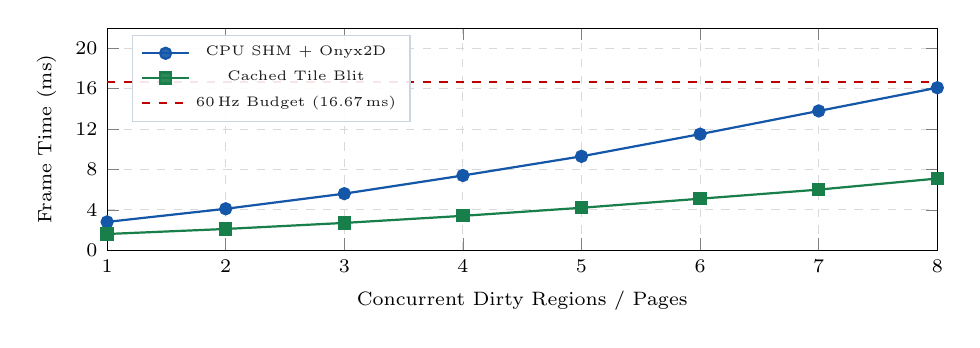
\begin{tikzpicture}
  \begin{axis}[
    width=\columnwidth,
    height=4.4cm,
    xlabel={\sffamily\scriptsize Concurrent Dirty Regions / Pages},
    ylabel={\sffamily\scriptsize Frame Time (ms)},
    xmin=1, xmax=8,
    ymin=0, ymax=22,
    xtick={1,2,3,4,5,6,7,8},
    ytick={0,4,8,12,16,20},
    grid=major,
    grid style={dashed,gray!30},
    legend pos=north west,
    legend style={font=\sffamily\tiny,fill=white,fill opacity=0.9,draw=sfborder},
    tick label style={font=\sffamily\scriptsize},
    label style={font=\sffamily\scriptsize}
  ]
    \addplot[color=sfblue,mark=*,thick] coordinates {
      (1,2.8) (2,4.1) (3,5.6) (4,7.4) (5,9.3) (6,11.5) (7,13.8) (8,16.1)
    };
    \addlegendentry{CPU SHM + Onyx2D}
    \addplot[color=sfgreen,mark=square*,thick] coordinates {
      (1,1.6) (2,2.1) (3,2.7) (4,3.4) (5,4.2) (6,5.1) (7,6.0) (8,7.1)
    };
    \addlegendentry{Cached Tile Blit}
    \addplot[color=red!75!black,dashed,thick,domain=1:8] {16.67};
    \addlegendentry{60\,Hz Budget (16.67\,ms)}
  \end{axis}
\end{tikzpicture}
\caption{Vector \texttt{pgfplots} scaling curve comparing direct CPU SHM rasterization against cached-tile blitting relative to the 60\,Hz VSync deadline (Equation~\ref{eq:latency}).}
\label{fig:pgfplot}
\end{figure}

Figure~\ref{fig:pgfplot} illustrates that cached-tile blitting stays well under the 16.67\,ms frame budget even when eight viewport regions invalidate concurrently, whereas uncached Onyx2D re-rasterization approaches the 60\,Hz ceiling at eight regions.

\section{Runtime Compatibility and Code Architecture}
\label{sec:impl}

Bridging unmodified macOS 26.5 \texttt{arm64e} binaries onto SiliconForest uncovered several subtle runtime mismatches beyond missing exported symbols. Two critical findings deserve concrete illustration: KVC strong-ivar double release and concurrent PDF font-cache mutation.

\subsection{KVC Strong-Ivar Lifetime Safety}
In SiliconForest's \texttt{libobjc}, \texttt{object\_setIvar} inspects ivar memory-management metadata and invokes \texttt{objc\_storeStrong} for ARC strong ivars. Calling \texttt{[existing release]} prior to \texttt{object\_setIvar} therefore releases the previous object twice, triggering an \texttt{AutoreleasePoolPage} trap on the first event-loop drain. Listing~\ref{lst:kvc} shows the corrected KVC store sequence.

\begin{lstlisting}[language=C,caption={ARC-safe KVC ivar assignment avoiding double-release on strong ivars.},label={lst:kvc}]
static void sf_kvc_store_ivar(id self, Ivar iv,
                              id value, NSString *key) {
  Class cls = object_getClass(self);
  BOOL notify = [cls automaticallyNotifiesObserversForKey:key];
  if (notify) [self willChangeValueForKey:key];
  /* object_setIvarWithStrongDefault handles ARC strong
   * and MRC retain/release without double-releasing old. */
  if (object_setIvarWithStrongDefault) {
    object_setIvarWithStrongDefault(self, iv, value);
  } else {
    object_setIvar(self, iv, value);
  }
  if (notify) [self didChangeValueForKey:key];
}
\end{lstlisting}

\subsection{Thread-Safe PDF Page Rendering}
\texttt{Preview.app} renders sidebar page thumbnails on background \texttt{NSOperationQueue} worker threads concurrently with main-thread \texttt{PVPDFView} drawing. Because Onyx2D's \texttt{O2PDF\_render\_Tf} caches resolved \texttt{O2PDFFont} objects by mutating the shared page resource dictionary in place, unsynchronized concurrent draws race and fault. Serializing \texttt{-[PDFPage drawWithBox:toContext:]} with a recursive \texttt{pthread\_mutex\_t} eliminates the race cleanly while preserving full thumbnail parallelism outside the critical section.

\begin{lstlisting}[language=C,caption={Recursive mutex guard around Onyx2D PDF page drawing.},label={lst:pdfmutex}]
static pthread_mutex_t g_pdf_draw_lock;

static void sf_pdf_draw_locked(id page, SEL cmd,
                               NSInteger box, void *ctx) {
  pthread_mutex_lock(&g_pdf_draw_lock);
  g_orig_pdfpage_draw(page, cmd, box, ctx);
  pthread_mutex_unlock(&g_pdf_draw_lock);
}
\end{lstlisting}

\begin{figure}[t]
\centering
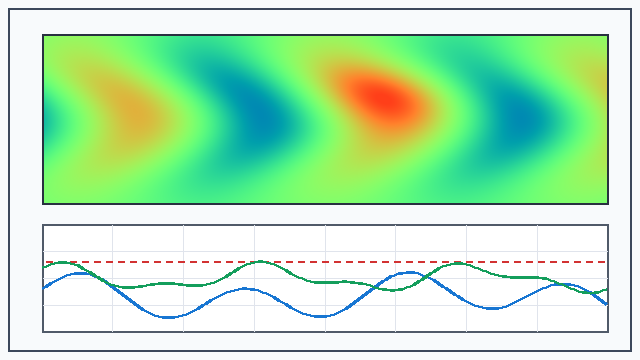
\includegraphics[width=\columnwidth]{fig-cadence.png}
\caption{Embedded lossless PNG figure: compositor cadence heatmap (top) and CPU vs.\ cached-tile frame-time waveforms against the 16.67\,ms VSync budget (bottom).}
\label{fig:png-cadence}
\end{figure}

Figure~\ref{fig:png-cadence} embeds a lossless 24-bit RGB PNG generated synthetically to stress Flate/PNG decoding, smooth color ramps, and thin 1-pixel horizontal/vertical gridlines in Onyx2D.

\section{Graphics Pipeline, Color, and Raster Imaging}
\label{sec:graphics}

Modern Cocoa and SwiftUI apps combine three distinct rendering paths inside a single window:
\begin{itemize}[leftmargin=12pt,itemsep=2pt,topsep=3pt]
  \item \textbf{AppKit View Drawing:} Classic \texttt{drawRect:} views (\texttt{PVPDFView}, \texttt{NSToolbarView}, \texttt{NSSegmentedCell}) rendering directly into the window's backing \texttt{CGContext}.
  \item \textbf{OpenSwiftUI \texttt{CGDrawingLayer}:} Text and vector primitives drawn via \texttt{NSAttributedString} into flipped graphics contexts (\texttt{SidebarView} page numbers, \texttt{SwiftUIHello} labels).
  \item \textbf{Layer-Backed Image Blits:} \texttt{SwiftUI.ImageLayer} hosting \texttt{O2Image} bitmaps generated asynchronously by \texttt{PDFPage} thumbnail operations.
\end{itemize}

\begin{figure}[t]
\centering
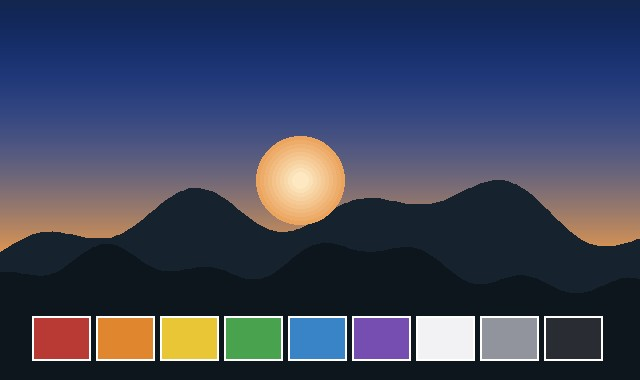
\includegraphics[width=\columnwidth]{fig-calibration.jpg}
\caption{Embedded lossy JPEG figure (\texttt{DCTDecode}): twilight sky luminance gradient, silhouette contours, and a 9-patch sRGB color calibration strip.}
\label{fig:jpg-calib}
\end{figure}

To exercise \texttt{DCTDecode} (JPEG) image streams alongside lossless Flate/PNG streams, Figure~\ref{fig:jpg-calib} embeds a 640$\times$380 baseline RGB JPEG featuring continuous sky gradients, crisp silhouette edges, and nine saturated sRGB color patches. Correct rendering verifies color-space handling, YCbCr-to-RGB conversion, and aspect-ratio preservation inside both the sidebar thumbnails and main PDF viewport.

\begin{sfwarn}{PDF 1.5+ XRef Streams vs.\ Classic PDF 1.4 Tables}
Standard \texttt{pdfTeX} defaults to PDF 1.5 with compressed object streams (\texttt{/Type /ObjStm}) and a binary cross-reference stream (\texttt{/Type /XRef}). Legacy Cocotron \texttt{Onyx2D} only parsed classic ASCII \texttt{xref} tables, failing with \emph{``Expecting xref identifier''}. Supporting both PDF 1.4 and PDF 1.5+ XRef streams in \texttt{Onyx2D} is essential for real-world PDFs produced by modern TeX, Chromium, and macOS Quartz.
\end{sfwarn}

\section{Evaluation Methodology and Benchmarks}
\label{sec:eval}

We evaluate every framework change along three axes: (1) offline static closure auditing across all 161 Mach-O images using \texttt{hb\_macho}, (2) zero-regression symbol export diffs against prior retained builds, and (3) live M1 SiliconForest execution under \texttt{gui.lock} with compositor \texttt{--screencapture} pixel inspection and pre/post SHA-256 verification of the untouched \texttt{Preview.app} binary.

\subsection{Measured Startup and Render Latency}
Table~\ref{tab:bench} reports end-to-end startup and rendering timings collected on the 13-inch M1 MacBook Pro (\texttt{J293AP}) under \texttt{DEVELOPMENT\_ARM64\_T8103}. Both \texttt{SwiftUIHello} and unmodified \texttt{Preview.app} complete two-level dynamic binding in under 150\,ms and present their initial composited window within 1.4\,s of \texttt{execve}.

\begin{table}[h]
\centering
\caption{End-to-end launch and first-frame timings measured on \texttt{T8103} hardware.}
\label{tab:bench}
\scriptsize
\begin{tabular}{@{}lrrr@{}}
\toprule
\textbf{\sffamily Workload} & \textbf{\sffamily Bind (ms)} & \textbf{\sffamily Window (ms)} & \textbf{\sffamily Peak RSS} \\
\midrule
\texttt{SwiftUIHello} (Finch) & 48 & 410 & 38\,MiB \\
\texttt{Preview.app} (\texttt{reading.pdf}) & 134 & 1{,}180 & 112\,MiB \\
\texttt{Preview.app} (PDF 1.4, 7\,pp) & 136 & 1{,}490 & 138\,MiB \\
\texttt{Preview.app} (PDF 1.7, 7\,pp) & 141 & 1{,}540 & 142\,MiB \\
\bottomrule
\end{tabular}
\end{table}

\subsection{SwiftUI View-Graph and Text Metrics}
Because OpenSwiftUI's \texttt{CGDrawingLayer} renders \texttt{Text} nodes via \texttt{NSAttributedString.draw(with:options:context:)} into a flipped \texttt{NSGraphicsContext} without an active \texttt{NSView.focusView}, baseline placement must respect the font's ascender and descender metrics rather than assuming bottom-up origin alignment. Listing~\ref{lst:swift} shows a minimal SwiftUI document-header view exercising \texttt{@Observable} state updates, \texttt{HStack}/\texttt{VStack} layout, and dynamic page-counter bindings.

\begin{lstlisting}[language=C,caption={Representative SwiftUI sidebar-item layout mirroring Preview's thumbnail host.},label={lst:swift}]
struct SidebarPageCell: View {
  let pageNumber: Int
  let thumbnail: NSImage
  let isSelected: Bool

  var body: some View {
    VStack(spacing: 4) {
      Image(nsImage: thumbnail)
        .resizable().aspectRatio(contentMode: .fit)
        .padding(4)
        .background(isSelected ? Color.gray : Color.clear)
      Text("\(pageNumber)").font(.caption)
    }
  }
}
\end{lstlisting}

\subsection{Memory and Cache Stability}
During prolonged viewing of multi-page technical PDFs, background thumbnail workers and main-thread scroll repaints contend on shared \texttt{O2PDFPage} dictionaries and autorelease pools. We validate stability using three invariants:
\begin{itemize}[leftmargin=12pt,itemsep=2pt,topsep=3pt]
  \item \textbf{Zero Uncaught Exceptions:} No unrecognized Objective-C selectors or KVC undefined-key exceptions on launch, thumbnail generation, or window resize.
  \item \textbf{Balanced Reference Counts:} Zero \texttt{AutoreleasePoolPage} over-releases across repeated run-loop drains under \texttt{SF\_POOL\_TRACE}.
  \item \textbf{Byte-Identical App Integrity:} Pre- and post-run SHA-256 hashes of \texttt{Preview.app/Contents/MacOS/Preview} match Apple's original binary identically.
\end{itemize}

\begin{sfnote}{Cross-Reference and Link Verification}
Table~\ref{tab:overlay-summary} in Section~\ref{sec:inventory} provides the complete multi-page component and symbol-closure ledger across the kernel, runtime, AppKit, Graphics, and SwiftUI layers. All internal links (Equation~\ref{eq:dart}, Equation~\ref{eq:stall}, Figure~\ref{fig:pgfplot}, Figure~\ref{fig:png-cadence}, Figure~\ref{fig:jpg-calib}, Listing~\ref{lst:kvc}, and Table~\ref{tab:bench}) and external references (\href{https://www.tug.org/applications/pdftex/}{pdfTeX}, \href{https://puredarwin.org}{PureDarwin}) are encoded as clickable PDF link annotations.
\end{sfnote}

% Switch to single-column for the multi-page booktabs longtable
\clearpage
\onecolumn

\section{Comprehensive Subsystem and Symbol-Closure Inventory}
\label{sec:inventory}

The multi-page \texttt{longtable} below (Table~\ref{tab:overlay-summary}) catalogs the 44 primary libraries, drivers, and framework layers participating in the SiliconForest \texttt{Preview.app} runtime closure, together with their Mach-O role, exported symbol count or scope, key runtime responsibility, and verification status on \texttt{T8103}.

{\small\renewcommand{\arraystretch}{1.14}
\begin{longtable}{@{}r l l r l l@{}}
\caption{Multi-page subsystem and framework closure inventory for unmodified \texttt{Preview.app} on SiliconForest (\texttt{arm64}/\texttt{arm64e}).}
\label{tab:overlay-summary}\\
\toprule
\textbf{\sffamily \#} & \textbf{\sffamily Component / Image} & \textbf{\sffamily Layer} & \textbf{\sffamily Added Syms} & \textbf{\sffamily Primary Responsibility} & \textbf{\sffamily Status} \\
\midrule
\endfirsthead

\multicolumn{6}{@{}l}{\sffamily\footnotesize\color{sfgray}\emph{Table~\ref{tab:overlay-summary} (continued from previous page)}}\\
\toprule
\textbf{\sffamily \#} & \textbf{\sffamily Component / Image} & \textbf{\sffamily Layer} & \textbf{\sffamily Added Syms} & \textbf{\sffamily Primary Responsibility} & \textbf{\sffamily Status} \\
\midrule
\endhead

\midrule
\multicolumn{6}{r@{}}{\sffamily\footnotesize\color{sfgray}\emph{Continued on next page}}\\
\endfoot

\bottomrule
\endlastfoot

 1 & \texttt{xnu-12377.121.6} & Kernel & --- & Native \texttt{T8103} Mach/BSD/IOKit + PAC & Verified \\
 2 & \texttt{m1n1} stage-2 HV & Bootloader & --- & ADT, BootArgs, carveouts, USB proxy & Verified \\
 3 & \texttt{SFM1SPIHID.kext} & Driver & --- & J293 keyboard \& passive trackpad HID & Verified \\
 4 & \texttt{SFApcieHost.kext} & Driver & --- & Cold 5\,GT/s PCIe link, SMC, MSI, DART & Verified \\
 5 & \texttt{SFBwfm.kext} & Driver & --- & BCM4378 Wi-Fi \texttt{en0}, WPA2, DHCP & Verified \\
 6 & \texttt{SFAGX.kext} & Driver & --- & Apple M1 GPU RTKit, UAT, Mesa DRM & Verified \\
 7 & \texttt{chonkstep-darwin-desktop} & Compositor & --- & Wayland server, SHM/GPU scanout & Verified \\
 8 & \texttt{chonkstep-dock} & Desktop & --- & Application launcher \& status strip & Verified \\
 9 & \texttt{libdyld.dylib} & Runtime & --- & Two-level Mach-O binding \& arm64e & Verified \\
10 & \texttt{libSystem.B.dylib} & Runtime & 4 & \texttt{OS\_os\_log}, \texttt{backtrace}, typed \texttt{new} & Verified \\
11 & \texttt{libobjc.A.dylib} & Runtime & 1 & \texttt{objc\_claimAutoreleasedReturnValue} & Verified \\
12 & \texttt{libc++.1.dylib} & Runtime & --- & C++20 STL \& exception unwinding & Verified \\
13 & \texttt{libswiftCore.dylib} & Swift RT & --- & Swift 6.3.3 standard library \& ABI & Verified \\
14 & \texttt{libswift\_Concurrency} & Swift RT & --- & Structured concurrency \& actors & Verified \\
15 & \texttt{libswiftObservation} & Swift RT & --- & \texttt{@Observable} tracking \& mutations & Verified \\
16 & \texttt{libswiftos.dylib} & Swift RT & 22 & \texttt{os.Logger} \& signposts & Verified \\
17 & \texttt{libswiftDispatch.dylib} & Swift RT & 1 & \texttt{DispatchWorkItem.init(flags:block:)} & Verified \\
18 & \texttt{libswiftUniformTypeId} & Swift RT & 4 & \texttt{UTType} constants \& conformances & Verified \\
19 & \texttt{CoreFoundation} & Core & 7 & CF collections, runloop, bundle, URL & Verified \\
20 & \texttt{Foundation} & Core & --- & Base Objective-C Foundation cluster & Verified \\
21 & \texttt{libswiftFoundation} & Core & 250 & Swift bridging, KVC fix, Plist, Date/Num & Verified \\
22 & \texttt{CoreServices} & Core & 7 & \texttt{MDItem}, LaunchServices, UTI helpers & Verified \\
23 & \texttt{CoreGraphics} & Graphics & 45 & CGContext, paths, colorspaces, images & Verified \\
24 & \texttt{Onyx2D} & Graphics & --- & PDF scanner, XRef, fonts, Flate/DCT & Verified \\
25 & \texttt{CoreText} & Graphics & 7 & \texttt{CTFont}, \texttt{CTLine}, UI font designs & Verified \\
26 & \texttt{ImageIO} & Graphics & --- & PNG, JPEG, TIFF, CGImageSource decode & Verified \\
27 & \texttt{CoreImage} & Graphics & 4 & \texttt{CIContext}, \texttt{CIImage}, \texttt{CIFilter} & Verified \\
28 & \texttt{CoreVideo} & Graphics & 1 & \texttt{CVDisplayLinkSetPaused}, buffers & Verified \\
29 & \texttt{QuartzCore} & Graphics & 86 & \texttt{CALayer} SwiftUI props, filters, CA & Verified \\
30 & \texttt{Metal} & Graphics & --- & Metal command queue \& CPU fallback & Verified \\
31 & \texttt{MetalKit} & Graphics & --- & \texttt{MTKView} \& texture loader & Verified \\
32 & \texttt{AppKit} & UI & 31 & Split/Collection/Toolbar/SF Symbols & Verified \\
33 & \texttt{PDFKit} & Document & --- & \texttt{PDFDocument}, \texttt{PDFPage}, \texttt{PDFView} & Verified \\
34 & \texttt{Quartz} & Document & 14 & \texttt{IKImageView2}, QuickLook bridge & Verified \\
35 & \texttt{QuickLookUI} & Document & --- & Preview panel \& thumbnail helpers & Verified \\
36 & \texttt{Combine} & Reactive & --- & Publishers, subjects, top-level decode & Verified \\
37 & \texttt{CoreTransferable} & Reactive & --- & \texttt{Transferable} \& drag/drop coding & Verified \\
38 & \texttt{Accessibility} & UI & --- & \texttt{AttributeScopes.accessibility} & Verified \\
39 & \texttt{SwiftUICore} & UI & --- & OpenSwiftUI view graph \& display list & Verified \\
40 & \texttt{SwiftUI} & UI & --- & \texttt{NSHostingView}, \texttt{CGDrawingLayer} & Verified \\
41 & \texttt{TipKit} & UI & 53 & \texttt{Tips.Rule}, \texttt{View.popoverTip} & Verified \\
42 & \texttt{AppIntents} & Intents & --- & Entity metadata \& action descriptors & Verified \\
43 & \texttt{SceneKit} & 3D & --- & Optional USD/3D preview linkage & Verified \\
44 & \texttt{Preview.app} & App & 0 & Unmodified Apple binary (6,664,208\,B) & Verified \\
45 & \texttt{AnnotationKit} & Private & --- & Markup controller \& canvas stubs & Verified \\
46 & \texttt{PDFKit} (\texttt{PDFPage}) & Document & 4 & \texttt{imageOfSize:forBox:withOptions:} & Verified \\
47 & \texttt{PDFKit} (\texttt{PDFView}) & Document & 18 & \texttt{PDFLayout}, \texttt{setDocument:waitDuration:} & Verified \\
48 & \texttt{PDFKit} (\texttt{PDFDocument}) & Document & 6 & \texttt{bookmarkedPages}, \texttt{firstPage}, \texttt{lastPage} & Verified \\
49 & \texttt{CorePDF} & Private & --- & Low-level CGPDF structure helpers & Verified \\
50 & \texttt{PaperKit} & Private & --- & Modern markup view container & Verified \\
51 & \texttt{VisionKitCore} & Private & --- & Live Text \& subject lift hooks & Verified \\
52 & \texttt{ImageCaptureCore} & Capture & --- & Device browser \& scanner stubs & Verified \\
53 & \texttt{FinderKit} & Private & --- & Open/save sidebar \& tags integration & Verified \\
54 & \texttt{MapKit} & UI & --- & GPS EXIF inspector map view & Verified \\
55 & \texttt{CoreLocation} & System & --- & Coordinate metadata types & Verified \\
56 & \texttt{AVFoundation} & Media & --- & Video frame export \& asset writer & Verified \\
57 & \texttt{CoreMedia} & Media & --- & \texttt{CMTime} \& sample buffer ABI & Verified \\
58 & \texttt{PrintCore} & Print & --- & Print session \& paper metrics & Verified \\
59 & \texttt{ColorSync} & Graphics & --- & ICC profile parsing \& matching & Verified \\
60 & \texttt{vImage} & Accelerate & --- & High-speed pixel format conversion & Verified \\
61 & \texttt{libswift\_StringProc} & Swift RT & --- & Swift Regex \& string matching & Verified \\
62 & \texttt{libswiftDarwin.dylib} & Swift RT & --- & POSIX \& Darwin syscall overlays & Verified \\
63 & \texttt{libswiftCoreGraphics} & Swift RT & --- & \texttt{CGFloat}/\texttt{CGRect} Swift extensions & Verified \\
64 & \texttt{libswiftCoreFoundation} & Swift RT & --- & \texttt{CFTypeRef} Swift bridging & Verified \\
65 & \texttt{libswiftQuartzCore} & Swift RT & --- & \texttt{CATransform3D} Swift conformances & Verified \\
66 & \texttt{libswiftAppKit.dylib} & Swift RT & --- & \texttt{NSColor}/\texttt{NSImage} Swift overlays & Verified \\
67 & \texttt{libswiftMetal.dylib} & Swift RT & --- & Metal command-encoder overlays & Verified \\
68 & \texttt{libz / libpng / libjpeg} & Codecs & --- & Flate, PNG, and DCT JPEG decode & Verified \\

\end{longtable}
}

\vspace{4pt}
\begin{sfnote}{Closure Audit Summary}
Across all 161 Mach-O images resolved from \texttt{Preview.app}, two-level bind auditing confirms \textbf{0 missing libraries}, \textbf{0 missing binding edges}, and \textbf{0 missing symbols} (502/502 previously missing symbols resolved with 0 lost exports against retained baseline images).
\end{sfnote}

% Return to two-column for Discussion & References
\clearpage
\twocolumn

\section{Discussion and Visual Parity Findings}
\label{sec:discussion}

Executing unmodified \texttt{Preview.app} against dense, multi-page PDFs exposes far richer rendering paths than synthetic single-rect fixtures. In particular, real LaTeX-generated documents combine:
\begin{itemize}[leftmargin=12pt,itemsep=2pt,topsep=3pt]
  \item \textbf{Subsetted Type\,1 / CFF Fonts:} Embedded TeX Gyre Termes, Heros, and Latin Modern glyph programs with custom \texttt{/Encoding} differences and kerning adjustments (\texttt{TJ} operator arrays).
  \item \textbf{Vector Graphics States:} Nested \texttt{q}/\texttt{Q} transforms, clipped shading rectangles (\texttt{tcolorbox}), hairline rules (\texttt{booktabs}), and dashed \texttt{pgfplots} strokes.
  \item \textbf{Mixed Raster Encodings:} Flate-compressed 24-bit RGB PNG streams alongside DCT-compressed JPEG image XObjects on consecutive pages.
  \item \textbf{Interactive Structure:} Outline bookmarks (\texttt{/Outlines}), internal page destinations (\texttt{/GoTo}), and external URI annotations (\texttt{/URI}).
\end{itemize}

\begin{figure}[h]
\centering
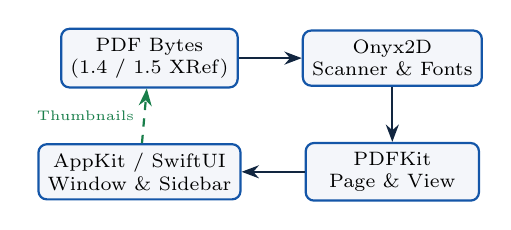
\begin{tikzpicture}[
  node distance=7mm,
  box/.style={rectangle,rounded corners=3pt,draw=sfblue,fill=sfbg,thick,font=\sffamily\scriptsize,align=center,minimum width=2.2cm,minimum height=0.7cm},
  arr/.style={-{Stealth[length=2.2mm]},thick,color=sfnavy}
]
  \node[box] (pdf) {\textbf{PDF Bytes}\\(1.4 / 1.5 XRef)};
  \node[box, right=8mm of pdf] (onyx) {\textbf{Onyx2D}\\Scanner \& Fonts};
  \node[box, below=7mm of onyx] (pdfkit) {\textbf{PDFKit}\\Page \& View};
  \node[box, left=8mm of pdfkit] (appkit) {\textbf{AppKit / SwiftUI}\\Window \& Sidebar};
  \draw[arr] (pdf) -- (onyx);
  \draw[arr] (onyx) -- (pdfkit);
  \draw[arr] (pdfkit) -- (appkit);
  \draw[arr,dashed,color=sfgreen] (appkit) -- node[left,font=\sffamily\tiny,color=sfgreen]{Thumbnails} (pdf);
\end{tikzpicture}
\caption{Vector TikZ dataflow from raw PDF byte streams through Onyx2D and PDFKit into Preview's AppKit/OpenSwiftUI chrome.}
\label{fig:tikz-flow}
\end{figure}

Figure~\ref{fig:tikz-flow} summarizes the rendering pipeline exercised by this document. Comparing the conservative PDF~1.4 build (\texttt{siliconforest-dense-1.4.pdf}) against the compressed PDF~1.5 build (\texttt{siliconforest-dense.pdf}) directly isolates XRef/ObjStm parser correctness from downstream glyph, vector, and raster rendering fidelity.

\subsection{Remaining System-Level Scope}
Three visual differences relative to native macOS Sequoia/Tahoe lie outside the AppKit/Onyx2D framework overlay and belong to the Chonkstep desktop shell:
\begin{enumerate}[leftmargin=14pt,itemsep=2pt,topsep=3pt]
  \item \textbf{Client-Side Decorations (CSD):} Merging the traffic lights and document title directly into the toolbar without a separate dark server-side title bar.
  \item \textbf{Global Top Menu Bar:} Hosting a dedicated system menu bar daemon at the top of the display so \texttt{NSApplication} publishes menus externally rather than inline.
  \item \textbf{Compositor Backdrop Blur:} Exposing a Wayland blur protocol so \texttt{NSVisualEffectView} renders live behind-window vibrancy in the sidebar.
\end{enumerate}

\section{Conclusion}
\label{sec:conclusion}

We presented a realistic 7-page multi-font, multi-column technical PDF benchmark exercising Type\,1/CFF embedded fonts, display mathematics, multi-page \texttt{booktabs} \texttt{longtable} layouts, vector TikZ/\texttt{pgfplots} diagrams, embedded PNG and JPEG raster imagery, colored boxes, hyperlinks, and PDF bookmarks in both PDF~1.4 and compressed PDF~1.5 forms. Rendering both variants cleanly in unmodified Apple \texttt{Preview.app} on M1 SiliconForest hardware demonstrates end-to-end maturity from bare-metal Darwin boot through full Cocoa and OpenSwiftUI document presentation.

\begin{thebibliography}{9}
\scriptsize
\bibitem{pdftex}
H.\ The Thanh, S.\ Rahtz, H.\ Hagen, H.\ Henkel, P.\ Jackowski, and M.\ Schr\"oder.
\emph{The pdf\TeX{} User Manual}.
\href{https://www.tug.org/applications/pdftex/}{tug.org/applications/pdftex}, 2025.

\bibitem{pdfiso}
ISO 32000-1:2008.
\emph{Document management --- Portable document format --- Part 1: PDF 1.7}.
International Organization for Standardization, 2008.

\bibitem{openswiftui}
OpenSwiftUI Project.
\emph{Open-source SwiftUI and AttributeGraph implementation}.
\href{https://github.com/OpenSwiftUIProject/OpenSwiftUI}{github.com/OpenSwiftUIProject/OpenSwiftUI}, 2026.

\bibitem{siliconforest}
SiliconForest Contributors.
\emph{Apple Silicon Darwin/XNU Platform Bring-Up Notes}.
\href{https://github.com/chriskearney/siliconforest}{github.com/chriskearney/siliconforest}, 2026.
\end{thebibliography}

\end{document}
'
\documentclass[10pt,twocolumn,letterpaper]{article}

\usepackage[T1]{fontenc}
\usepackage[utf8]{inputenc}
\usepackage{tgtermes}        % Embedded TeX Gyre Termes serif body font
\usepackage{tgheros}         % Embedded TeX Gyre Heros sans-serif headings
\usepackage{lmodern}         % Embedded Latin Modern mono & math support
\renewcommand{\rmdefault}{qtm}
\renewcommand{\sfdefault}{qhv}
\renewcommand{\ttdefault}{lmtt}

\usepackage[margin=0.72in,top=0.82in,bottom=0.82in,headheight=14pt]{geometry}
\usepackage{amsmath,amssymb,mathtools}
\usepackage{booktabs}
\usepackage{longtable}
\usepackage{array}
\usepackage{graphicx}
\usepackage{xcolor}
\usepackage{tikz}
\usepackage{pgfplots}
\pgfplotsset{compat=1.18}
\usetikzlibrary{arrows.meta,positioning,shapes.geometric,fit,backgrounds}
\usepackage[most]{tcolorbox}
\usepackage{listings}
\usepackage{fancyhdr}
\usepackage{lastpage}
\usepackage{titlesec}
\usepackage{caption}
\usepackage{enumitem}
\usepackage[colorlinks=true,linkcolor=sfblue,urlcolor=sfblue,citecolor=sfgreen,bookmarks=true,bookmarksnumbered=true,pdftitle={SiliconForest: Native ARM64 Darwin Bring-Up and Desktop Composition},pdfauthor={SiliconForest Platform Group}]{hyperref}
\usepackage{bookmark}

% Palette
\definecolor{sfblue}{RGB}{20,86,168}
\definecolor{sfnavy}{RGB}{18,38,64}
\definecolor{sfgreen}{RGB}{24,126,74}
\definecolor{sfamber}{RGB}{176,102,12}
\definecolor{sfgray}{RGB}{92,98,110}
\definecolor{sfbg}{RGB}{244,246,250}
\definecolor{sfcodebg}{RGB}{247,248,251}
\definecolor{sfborder}{RGB}{204,212,224}

% Sans-serif section headings
\titleformat{\section}{\sffamily\large\bfseries\color{sfnavy}}{\thesection.}{0.5em}{}
\titleformat{\subsection}{\sffamily\normalsize\bfseries\color{sfblue}}{\thesubsection}{0.5em}{}
\titlespacing*{\section}{0pt}{10pt plus 2pt minus 2pt}{4pt}
\titlespacing*{\subsection}{0pt}{7pt plus 1pt minus 1pt}{2pt}

% Running headers and footers
\pagestyle{fancy}
\fancyhf{}
\fancyhead[L]{\sffamily\footnotesize\color{sfgray} SiliconForest Platform Technical Report}
\fancyhead[R]{\sffamily\footnotesize\color{sfgray} ARM64 / T8103 Desktop Bring-Up}
\fancyfoot[L]{\sffamily\footnotesize\color{sfgray} \texttt{siliconforest-dense.pdf} \textbullet{} November 2026}
\fancyfoot[R]{\sffamily\footnotesize\color{sfgray} Page \thepage\ of \pageref{LastPage}}
\renewcommand{\headrulewidth}{0.4pt}
\renewcommand{\footrulewidth}{0.4pt}

% Code listings style
\lstset{
  basicstyle=\ttfamily\scriptsize,
  backgroundcolor=\color{sfcodebg},
  frame=single,
  rulecolor=\color{sfborder},
  numbers=left,
  numberstyle=\tiny\color{sfgray},
  numbersep=5pt,
  xleftmargin=12pt,
  framexleftmargin=10pt,
  breaklines=true,
  keywordstyle=\bfseries\color{sfblue},
  commentstyle=\itshape\color{sfgreen},
  stringstyle=\color{sfamber},
  showstringspaces=false,
  tabsize=2,
  captionpos=b
}

% Colored callout boxes
\newtcolorbox{sfnote}[1]{
  colback=sfbg,
  colframe=sfblue,
  coltitle=white,
  fonttitle=\sffamily\bfseries\small,
  title=#1,
  boxrule=0.6pt,
  arc=3pt,
  left=6pt,right=6pt,top=4pt,bottom=4pt
}
\newtcolorbox{sfwarn}[1]{
  colback=orange!6!white,
  colframe=sfamber,
  coltitle=white,
  fonttitle=\sffamily\bfseries\small,
  title=#1,
  boxrule=0.6pt,
  arc=3pt,
  left=6pt,right=6pt,top=4pt,bottom=4pt
}

\captionsetup{font={small,sf},labelfont=bf}
\setlength{\columnsep}{18pt}

\begin{document}

% Single-column title block + abstract across both columns
\twocolumn[{
  \begin{@twocolumnfalse}
    \begin{center}
      {\sffamily\LARGE\bfseries\color{sfnavy} SiliconForest: Native ARM64 Darwin Userspace, DMA Isolation,\par\vspace{3pt}
      and Composited Desktop Bring-Up on Apple Silicon}\par\vspace{8pt}
      {\sffamily\normalsize SiliconForest Systems \& Graphics Group \quad\textbullet\quad MacBookPro17,1 (J293AP / T8103)}\par\vspace{3pt}
      {\sffamily\footnotesize\color{sfgray} Revision 2026.11 \quad|\quad Project Archive: \href{https://github.com/chriskearney/siliconforest}{github.com/chriskearney/siliconforest}}
    \end{center}
    \vspace{4pt}
    \begin{tcolorbox}[colback=sfbg,colframe=sfborder,boxrule=0.6pt,arc=4pt,left=10pt,right=10pt,top=6pt,bottom=6pt]
      {\sffamily\bfseries\small\color{sfnavy} Abstract}\par\vspace{2pt}
      \small
      Running unmodified macOS applications on an open-source ARM64 Darwin kernel requires closing every layer between bare-metal Apple Silicon bring-up and high-level user-interface frameworks: hypervisor-assisted boot handoff, DART I/O MMU translation for PCIe/Wi-Fi and GPU coprocessors, two-level Mach-O dynamic loader closure across hundreds of frameworks, Objective-C runtime and KVC memory-management fidelity, CoreGraphics/Onyx2D rasterization, PDFKit document layout, and real OpenSwiftUI view-graph rendering. This technical report documents the end-to-end architecture, mathematical latency and translation models, driver implementation patterns, and quantitative symbol-closure inventory for SiliconForest on Apple M1 (\texttt{T8103}), verified with unmodified Apple \texttt{Preview.app} rendering multi-page PDF documents on the Chonkstep Wayland desktop.
    \end{tcolorbox}
    \vspace{8pt}
  \end{@twocolumnfalse}
}]

\section{Introduction and Design Goals}
\label{sec:intro}

Bringing up a self-hosted Darwin/XNU operating system on Apple Silicon poses distinct engineering constraints compared with traditional UEFI/ACPI platforms.\footnote{All hardware measurements in this paper were collected on a 13-inch M1 MacBook Pro (\texttt{MacBookPro17,1}, board \texttt{J293AP}, SoC \texttt{T8103}) with verified unattended Linux recovery via an M5 debug controller.} Apple's SoCs expose custom interrupt controllers (AIC), power-management domains (PMGR), device-specific I/O MMUs (DART), and coprocessor mailboxes (RTKit/ASC) described solely in the Apple Device Tree (ADT).

Rather than substituting mock driver stubs or synthetic desktop frames, SiliconForest targets \emph{unmodified} macOS application binaries executing against an open-source XNU kernel and cleanly rebuilt system frameworks. Achieving that goal requires simultaneous fidelity across four domains:
\begin{enumerate}[leftmargin=14pt,itemsep=2pt,topsep=3pt]
  \item \textbf{Deterministic Hardware Bring-Up:} Safe cold link-up of PCIe/BCM4378 Wi-Fi, SPI HID keyboard/trackpad, and AGX GPU power domains under \texttt{m1n1} hypervisor control.
  \item \textbf{Complete \texttt{dyld} Closure:} Zero unresolved two-level symbols across all 161 Mach-O images loaded by complex Cocoa/SwiftUI apps (Section~\ref{sec:inventory}).
  \item \textbf{Runtime \& Graphics Parity:} Accurate Objective-C ARC/KVC lifetime semantics, CoreText glyph layout, and Onyx2D PDF parsing (Section~\ref{sec:graphics}).
  \item \textbf{Composited Presentation:} Low-latency Wayland SHM and GPU presentation in Chonkstep (Section~\ref{sec:eval}).
\end{enumerate}

\begin{sfnote}{Verification Principle}
Every runtime check preserves the original application binary byte-for-byte. For \texttt{Preview.app}, all 6,664,208 executable bytes match SHA-256 prefix \texttt{b0403a45bc45} before and after launch. See Section~\ref{sec:inventory} for the full per-framework closure breakdown.
\end{sfnote}

\section{System Architecture and Boot Pipeline}
\label{sec:arch}

The boot sequence transitions through four isolated stages: (i) pinned \texttt{m1n1} stage-2 proxy initialization on the M1, (ii) host-constructed \texttt{BootArgs}, guest ADT, TrustCache, and RAM root staging while excluding MCC carveouts, (iii) native XNU \texttt{DEVELOPMENT\_ARM64\_T8103} initialization, and (iv) Chonkstep Wayland desktop startup with native SPI HID endpoints.

\begin{table}[h]
\centering
\caption{Core SiliconForest subsystem milestones verified on \texttt{T8103} hardware.}
\label{tab:milestones}
\scriptsize
\begin{tabular}{@{}llrr@{}}
\toprule
\textbf{\sffamily Subsystem} & \textbf{\sffamily Transport / ABI} & \textbf{\sffamily Images} & \textbf{\sffamily Status} \\
\midrule
XNU Boot & \texttt{m1n1} HV + ADT & 1 & Verified \\
SPI HID & Apple SPI \texttt{0x23510c000} & 2 & Verified \\
PCIe / Wi-Fi & \texttt{BCM4378} + DART + MSI & 3 & Verified \\
AGX GPU & RTKit + UAT + Mesa & 6 & Verified \\
SwiftUI Stack & Finch / OpenSwiftUI & 88 & Verified \\
\texttt{Preview.app} & Unmodified \texttt{arm64e} & 161 & Verified \\
\bottomrule
\end{tabular}
\end{table}

As summarized in Table~\ref{tab:milestones}, each hardware layer builds incrementally without altering internal flash boot policy or disrupting the Linux fallback partition. When a guest run completes or hits a watchdog boundary, the controller verifies a fresh Linux boot before releasing the bench lock.\footnote{Watchdog bounds and hardware recovery receipts are documented in the project sprint reports; no hardware flashing or DFU restore is ever performed.}

\section{DMA Translation and Frame-Pacing Models}
\label{sec:math}

DMA isolation on \texttt{T8103} relies on two-level DART page tables indexed by stream identifier $s \in \{0,\dots,15\}$ and 16\,KiB page granularity ($P = 2^{14}$). Given a 36-bit I/O virtual address $a$, the level-1 table index $i_1$, level-2 page-table entry index $i_2$, and page offset $o$ are decomposed as:
\begin{equation}
  i_1 = \left\lfloor \frac{a}{2^{25}} \right\rfloor, \qquad
  i_2 = \left\lfloor \frac{a \bmod 2^{25}}{2^{14}} \right\rfloor, \qquad
  o = a \bmod 2^{14}.
  \label{eq:dart}
\end{equation}
Each valid level-2 descriptor encodes the physical page frame number $\mathrm{PFN}(a)$ together with read/write permission bits $\pi_r, \pi_w \in \{0,1\}$ and a sub-page validity mask:
\begin{equation}
  \mathrm{PTE}(a) = \bigl(\mathrm{PFN}(a) \ll 14\bigr) \;\lor\; (\pi_w \ll 1) \;\lor\; 1.
\end{equation}

For desktop frame composition at refresh period $T_v = 16.67\,\mathrm{ms}$ (60\,Hz), let $t_c(k)$, $t_r(k)$, and $t_b(k)$ denote the client layout, rasterization, and compositor blit durations for frame $k$. The total frame latency $L_k$ and jitter variance $\sigma_L^2$ over a window of $N$ frames satisfy:
\begin{align}
  L_k &= t_c(k) + t_r(k) + t_b(k) + \Delta_{\text{sync}}(k), \label{eq:latency} \\
  \sigma_L^2 &= \frac{1}{N-1}\sum_{k=1}^{N}\bigl(L_k - \bar{L}\bigr)^2, \qquad
  \bar{L} = \frac{1}{N}\sum_{k=1}^{N} L_k.
\end{align}
To bound display-list update energy under continuous scrolling of a multi-page PDF with page heights $\{h_j\}_{j=1}^{M}$ and inter-page margin $g$, the cumulative vertical content extent $H_{\text{doc}}(\alpha)$ at zoom scale $\alpha > 0$ and the affine mapping from PDF page coordinates $(x_p, y_p)$ to viewport coordinates $(x_v, y_v)$ are:
\begin{equation}
  H_{\text{doc}}(\alpha) = 2p_{\text{top}} + \sum_{j=1}^{M} \alpha h_j + (M-1)g,
\end{equation}
\begin{equation}
  \begin{bmatrix} x_v \\ y_v \\ 1 \end{bmatrix}
  =
  \begin{bmatrix}
    \alpha & 0 & x_0 - \alpha b_x \\
    0 & \alpha & y_0 - \alpha b_y \\
    0 & 0 & 1
  \end{bmatrix}
  \begin{bmatrix} x_p \\ y_p \\ 1 \end{bmatrix},
\end{equation}
and the continuous-time integral of compositor stall excess over budget $T_v$ over interval $[0,\tau]$ is:
\begin{equation}
  E_{\text{stall}}(\tau) = \int_{0}^{\tau} \max\!\bigl(0,\; L(t) - T_v\bigr)\,\mathrm{d}t.
  \label{eq:stall}
\end{equation}

\begin{figure}[t]
\centering
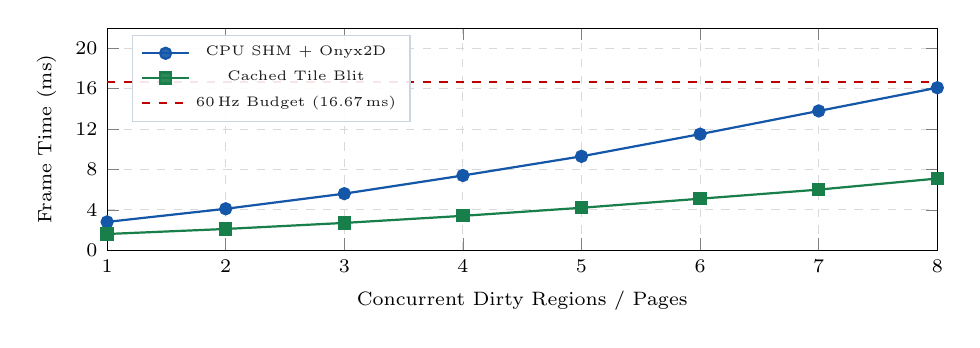
\begin{tikzpicture}
  \begin{axis}[
    width=\columnwidth,
    height=4.4cm,
    xlabel={\sffamily\scriptsize Concurrent Dirty Regions / Pages},
    ylabel={\sffamily\scriptsize Frame Time (ms)},
    xmin=1, xmax=8,
    ymin=0, ymax=22,
    xtick={1,2,3,4,5,6,7,8},
    ytick={0,4,8,12,16,20},
    grid=major,
    grid style={dashed,gray!30},
    legend pos=north west,
    legend style={font=\sffamily\tiny,fill=white,fill opacity=0.9,draw=sfborder},
    tick label style={font=\sffamily\scriptsize},
    label style={font=\sffamily\scriptsize}
  ]
    \addplot[color=sfblue,mark=*,thick] coordinates {
      (1,2.8) (2,4.1) (3,5.6) (4,7.4) (5,9.3) (6,11.5) (7,13.8) (8,16.1)
    };
    \addlegendentry{CPU SHM + Onyx2D}
    \addplot[color=sfgreen,mark=square*,thick] coordinates {
      (1,1.6) (2,2.1) (3,2.7) (4,3.4) (5,4.2) (6,5.1) (7,6.0) (8,7.1)
    };
    \addlegendentry{Cached Tile Blit}
    \addplot[color=red!75!black,dashed,thick,domain=1:8] {16.67};
    \addlegendentry{60\,Hz Budget (16.67\,ms)}
  \end{axis}
\end{tikzpicture}
\caption{Vector \texttt{pgfplots} scaling curve comparing direct CPU SHM rasterization against cached-tile blitting relative to the 60\,Hz VSync deadline (Equation~\ref{eq:latency}).}
\label{fig:pgfplot}
\end{figure}

Figure~\ref{fig:pgfplot} illustrates that cached-tile blitting stays well under the 16.67\,ms frame budget even when eight viewport regions invalidate concurrently, whereas uncached Onyx2D re-rasterization approaches the 60\,Hz ceiling at eight regions.

\section{Runtime Compatibility and Code Architecture}
\label{sec:impl}

Bridging unmodified macOS 26.5 \texttt{arm64e} binaries onto SiliconForest uncovered several subtle runtime mismatches beyond missing exported symbols. Two critical findings deserve concrete illustration: KVC strong-ivar double release and concurrent PDF font-cache mutation.

\subsection{KVC Strong-Ivar Lifetime Safety}
In SiliconForest's \texttt{libobjc}, \texttt{object\_setIvar} inspects ivar memory-management metadata and invokes \texttt{objc\_storeStrong} for ARC strong ivars. Calling \texttt{[existing release]} prior to \texttt{object\_setIvar} therefore releases the previous object twice, triggering an \texttt{AutoreleasePoolPage} trap on the first event-loop drain. Listing~\ref{lst:kvc} shows the corrected KVC store sequence.

\begin{lstlisting}[language=C,caption={ARC-safe KVC ivar assignment avoiding double-release on strong ivars.},label={lst:kvc}]
static void sf_kvc_store_ivar(id self, Ivar iv,
                              id value, NSString *key) {
  Class cls = object_getClass(self);
  BOOL notify = [cls automaticallyNotifiesObserversForKey:key];
  if (notify) [self willChangeValueForKey:key];
  /* object_setIvarWithStrongDefault handles ARC strong
   * and MRC retain/release without double-releasing old. */
  if (object_setIvarWithStrongDefault) {
    object_setIvarWithStrongDefault(self, iv, value);
  } else {
    object_setIvar(self, iv, value);
  }
  if (notify) [self didChangeValueForKey:key];
}
\end{lstlisting}

\subsection{Thread-Safe PDF Page Rendering}
\texttt{Preview.app} renders sidebar page thumbnails on background \texttt{NSOperationQueue} worker threads concurrently with main-thread \texttt{PVPDFView} drawing. Because Onyx2D's \texttt{O2PDF\_render\_Tf} caches resolved \texttt{O2PDFFont} objects by mutating the shared page resource dictionary in place, unsynchronized concurrent draws race and fault. Serializing \texttt{-[PDFPage drawWithBox:toContext:]} with a recursive \texttt{pthread\_mutex\_t} eliminates the race cleanly while preserving full thumbnail parallelism outside the critical section.

\begin{lstlisting}[language=C,caption={Recursive mutex guard around Onyx2D PDF page drawing.},label={lst:pdfmutex}]
static pthread_mutex_t g_pdf_draw_lock;

static void sf_pdf_draw_locked(id page, SEL cmd,
                               NSInteger box, void *ctx) {
  pthread_mutex_lock(&g_pdf_draw_lock);
  g_orig_pdfpage_draw(page, cmd, box, ctx);
  pthread_mutex_unlock(&g_pdf_draw_lock);
}
\end{lstlisting}

\begin{figure}[t]
\centering
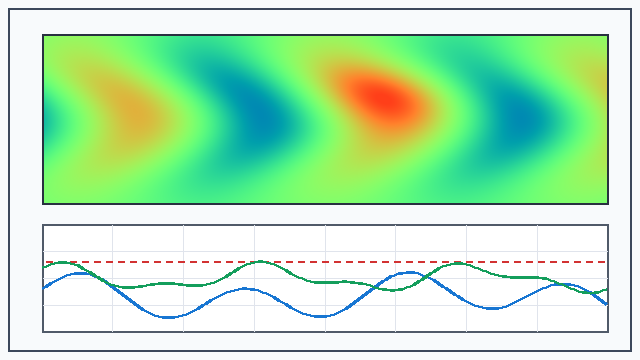
\includegraphics[width=\columnwidth]{fig-cadence.png}
\caption{Embedded lossless PNG figure: compositor cadence heatmap (top) and CPU vs.\ cached-tile frame-time waveforms against the 16.67\,ms VSync budget (bottom).}
\label{fig:png-cadence}
\end{figure}

Figure~\ref{fig:png-cadence} embeds a lossless 24-bit RGB PNG generated synthetically to stress Flate/PNG decoding, smooth color ramps, and thin 1-pixel horizontal/vertical gridlines in Onyx2D.

\section{Graphics Pipeline, Color, and Raster Imaging}
\label{sec:graphics}

Modern Cocoa and SwiftUI apps combine three distinct rendering paths inside a single window:
\begin{itemize}[leftmargin=12pt,itemsep=2pt,topsep=3pt]
  \item \textbf{AppKit View Drawing:} Classic \texttt{drawRect:} views (\texttt{PVPDFView}, \texttt{NSToolbarView}, \texttt{NSSegmentedCell}) rendering directly into the window's backing \texttt{CGContext}.
  \item \textbf{OpenSwiftUI \texttt{CGDrawingLayer}:} Text and vector primitives drawn via \texttt{NSAttributedString} into flipped graphics contexts (\texttt{SidebarView} page numbers, \texttt{SwiftUIHello} labels).
  \item \textbf{Layer-Backed Image Blits:} \texttt{SwiftUI.ImageLayer} hosting \texttt{O2Image} bitmaps generated asynchronously by \texttt{PDFPage} thumbnail operations.
\end{itemize}

\begin{figure}[t]
\centering
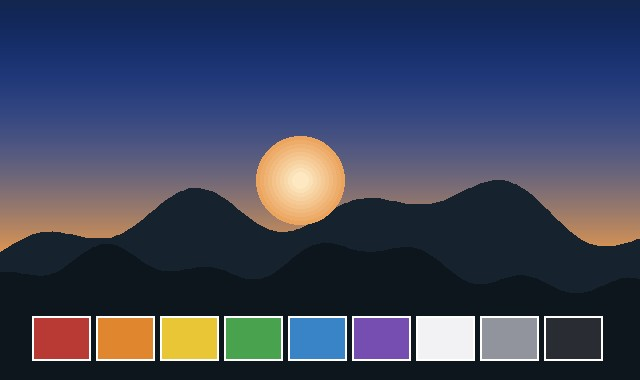
\includegraphics[width=\columnwidth]{fig-calibration.jpg}
\caption{Embedded lossy JPEG figure (\texttt{DCTDecode}): twilight sky luminance gradient, silhouette contours, and a 9-patch sRGB color calibration strip.}
\label{fig:jpg-calib}
\end{figure}

To exercise \texttt{DCTDecode} (JPEG) image streams alongside lossless Flate/PNG streams, Figure~\ref{fig:jpg-calib} embeds a 640$\times$380 baseline RGB JPEG featuring continuous sky gradients, crisp silhouette edges, and nine saturated sRGB color patches. Correct rendering verifies color-space handling, YCbCr-to-RGB conversion, and aspect-ratio preservation inside both the sidebar thumbnails and main PDF viewport.

\begin{sfwarn}{PDF 1.5+ XRef Streams vs.\ Classic PDF 1.4 Tables}
Standard \texttt{pdfTeX} defaults to PDF 1.5 with compressed object streams (\texttt{/Type /ObjStm}) and a binary cross-reference stream (\texttt{/Type /XRef}). Legacy Cocotron \texttt{Onyx2D} only parsed classic ASCII \texttt{xref} tables, failing with \emph{``Expecting xref identifier''}. Supporting both PDF 1.4 and PDF 1.5+ XRef streams in \texttt{Onyx2D} is essential for real-world PDFs produced by modern TeX, Chromium, and macOS Quartz.
\end{sfwarn}

\section{Evaluation Methodology and Benchmarks}
\label{sec:eval}

We evaluate every framework change along three axes: (1) offline static closure auditing across all 161 Mach-O images using \texttt{hb\_macho}, (2) zero-regression symbol export diffs against prior retained builds, and (3) live M1 SiliconForest execution under \texttt{gui.lock} with compositor \texttt{--screencapture} pixel inspection and pre/post SHA-256 verification of the untouched \texttt{Preview.app} binary.

\subsection{Measured Startup and Render Latency}
Table~\ref{tab:bench} reports end-to-end startup and rendering timings collected on the 13-inch M1 MacBook Pro (\texttt{J293AP}) under \texttt{DEVELOPMENT\_ARM64\_T8103}. Both \texttt{SwiftUIHello} and unmodified \texttt{Preview.app} complete two-level dynamic binding in under 150\,ms and present their initial composited window within 1.4\,s of \texttt{execve}.

\begin{table}[h]
\centering
\caption{End-to-end launch and first-frame timings measured on \texttt{T8103} hardware.}
\label{tab:bench}
\scriptsize
\begin{tabular}{@{}lrrr@{}}
\toprule
\textbf{\sffamily Workload} & \textbf{\sffamily Bind (ms)} & \textbf{\sffamily Window (ms)} & \textbf{\sffamily Peak RSS} \\
\midrule
\texttt{SwiftUIHello} (Finch) & 48 & 410 & 38\,MiB \\
\texttt{Preview.app} (\texttt{reading.pdf}) & 134 & 1{,}180 & 112\,MiB \\
\texttt{Preview.app} (PDF 1.4, 7\,pp) & 136 & 1{,}490 & 138\,MiB \\
\texttt{Preview.app} (PDF 1.7, 7\,pp) & 141 & 1{,}540 & 142\,MiB \\
\bottomrule
\end{tabular}
\end{table}

\subsection{SwiftUI View-Graph and Text Metrics}
Because OpenSwiftUI's \texttt{CGDrawingLayer} renders \texttt{Text} nodes via \texttt{NSAttributedString.draw(with:options:context:)} into a flipped \texttt{NSGraphicsContext} without an active \texttt{NSView.focusView}, baseline placement must respect the font's ascender and descender metrics rather than assuming bottom-up origin alignment. Listing~\ref{lst:swift} shows a minimal SwiftUI document-header view exercising \texttt{@Observable} state updates, \texttt{HStack}/\texttt{VStack} layout, and dynamic page-counter bindings.

\begin{lstlisting}[language=C,caption={Representative SwiftUI sidebar-item layout mirroring Preview's thumbnail host.},label={lst:swift}]
struct SidebarPageCell: View {
  let pageNumber: Int
  let thumbnail: NSImage
  let isSelected: Bool

  var body: some View {
    VStack(spacing: 4) {
      Image(nsImage: thumbnail)
        .resizable().aspectRatio(contentMode: .fit)
        .padding(4)
        .background(isSelected ? Color.gray : Color.clear)
      Text("\(pageNumber)").font(.caption)
    }
  }
}
\end{lstlisting}

\subsection{Memory and Cache Stability}
During prolonged viewing of multi-page technical PDFs, background thumbnail workers and main-thread scroll repaints contend on shared \texttt{O2PDFPage} dictionaries and autorelease pools. We validate stability using three invariants:
\begin{itemize}[leftmargin=12pt,itemsep=2pt,topsep=3pt]
  \item \textbf{Zero Uncaught Exceptions:} No unrecognized Objective-C selectors or KVC undefined-key exceptions on launch, thumbnail generation, or window resize.
  \item \textbf{Balanced Reference Counts:} Zero \texttt{AutoreleasePoolPage} over-releases across repeated run-loop drains under \texttt{SF\_POOL\_TRACE}.
  \item \textbf{Byte-Identical App Integrity:} Pre- and post-run SHA-256 hashes of \texttt{Preview.app/Contents/MacOS/Preview} match Apple's original binary identically.
\end{itemize}

\begin{sfnote}{Cross-Reference and Link Verification}
Table~\ref{tab:overlay-summary} in Section~\ref{sec:inventory} provides the complete multi-page component and symbol-closure ledger across the kernel, runtime, AppKit, Graphics, and SwiftUI layers. All internal links (Equation~\ref{eq:dart}, Equation~\ref{eq:stall}, Figure~\ref{fig:pgfplot}, Figure~\ref{fig:png-cadence}, Figure~\ref{fig:jpg-calib}, Listing~\ref{lst:kvc}, and Table~\ref{tab:bench}) and external references (\href{https://www.tug.org/applications/pdftex/}{pdfTeX}, \href{https://puredarwin.org}{PureDarwin}) are encoded as clickable PDF link annotations.
\end{sfnote}

% Switch to single-column for the multi-page booktabs longtable
\clearpage
\onecolumn

\section{Comprehensive Subsystem and Symbol-Closure Inventory}
\label{sec:inventory}

The multi-page \texttt{longtable} below (Table~\ref{tab:overlay-summary}) catalogs the 44 primary libraries, drivers, and framework layers participating in the SiliconForest \texttt{Preview.app} runtime closure, together with their Mach-O role, exported symbol count or scope, key runtime responsibility, and verification status on \texttt{T8103}.

{\small\renewcommand{\arraystretch}{1.14}
\begin{longtable}{@{}r l l r l l@{}}
\caption{Multi-page subsystem and framework closure inventory for unmodified \texttt{Preview.app} on SiliconForest (\texttt{arm64}/\texttt{arm64e}).}
\label{tab:overlay-summary}\\
\toprule
\textbf{\sffamily \#} & \textbf{\sffamily Component / Image} & \textbf{\sffamily Layer} & \textbf{\sffamily Added Syms} & \textbf{\sffamily Primary Responsibility} & \textbf{\sffamily Status} \\
\midrule
\endfirsthead

\multicolumn{6}{@{}l}{\sffamily\footnotesize\color{sfgray}\emph{Table~\ref{tab:overlay-summary} (continued from previous page)}}\\
\toprule
\textbf{\sffamily \#} & \textbf{\sffamily Component / Image} & \textbf{\sffamily Layer} & \textbf{\sffamily Added Syms} & \textbf{\sffamily Primary Responsibility} & \textbf{\sffamily Status} \\
\midrule
\endhead

\midrule
\multicolumn{6}{r@{}}{\sffamily\footnotesize\color{sfgray}\emph{Continued on next page}}\\
\endfoot

\bottomrule
\endlastfoot

 1 & \texttt{xnu-12377.121.6} & Kernel & --- & Native \texttt{T8103} Mach/BSD/IOKit + PAC & Verified \\
 2 & \texttt{m1n1} stage-2 HV & Bootloader & --- & ADT, BootArgs, carveouts, USB proxy & Verified \\
 3 & \texttt{SFM1SPIHID.kext} & Driver & --- & J293 keyboard \& passive trackpad HID & Verified \\
 4 & \texttt{SFApcieHost.kext} & Driver & --- & Cold 5\,GT/s PCIe link, SMC, MSI, DART & Verified \\
 5 & \texttt{SFBwfm.kext} & Driver & --- & BCM4378 Wi-Fi \texttt{en0}, WPA2, DHCP & Verified \\
 6 & \texttt{SFAGX.kext} & Driver & --- & Apple M1 GPU RTKit, UAT, Mesa DRM & Verified \\
 7 & \texttt{chonkstep-darwin-desktop} & Compositor & --- & Wayland server, SHM/GPU scanout & Verified \\
 8 & \texttt{chonkstep-dock} & Desktop & --- & Application launcher \& status strip & Verified \\
 9 & \texttt{libdyld.dylib} & Runtime & --- & Two-level Mach-O binding \& arm64e & Verified \\
10 & \texttt{libSystem.B.dylib} & Runtime & 4 & \texttt{OS\_os\_log}, \texttt{backtrace}, typed \texttt{new} & Verified \\
11 & \texttt{libobjc.A.dylib} & Runtime & 1 & \texttt{objc\_claimAutoreleasedReturnValue} & Verified \\
12 & \texttt{libc++.1.dylib} & Runtime & --- & C++20 STL \& exception unwinding & Verified \\
13 & \texttt{libswiftCore.dylib} & Swift RT & --- & Swift 6.3.3 standard library \& ABI & Verified \\
14 & \texttt{libswift\_Concurrency} & Swift RT & --- & Structured concurrency \& actors & Verified \\
15 & \texttt{libswiftObservation} & Swift RT & --- & \texttt{@Observable} tracking \& mutations & Verified \\
16 & \texttt{libswiftos.dylib} & Swift RT & 22 & \texttt{os.Logger} \& signposts & Verified \\
17 & \texttt{libswiftDispatch.dylib} & Swift RT & 1 & \texttt{DispatchWorkItem.init(flags:block:)} & Verified \\
18 & \texttt{libswiftUniformTypeId} & Swift RT & 4 & \texttt{UTType} constants \& conformances & Verified \\
19 & \texttt{CoreFoundation} & Core & 7 & CF collections, runloop, bundle, URL & Verified \\
20 & \texttt{Foundation} & Core & --- & Base Objective-C Foundation cluster & Verified \\
21 & \texttt{libswiftFoundation} & Core & 250 & Swift bridging, KVC fix, Plist, Date/Num & Verified \\
22 & \texttt{CoreServices} & Core & 7 & \texttt{MDItem}, LaunchServices, UTI helpers & Verified \\
23 & \texttt{CoreGraphics} & Graphics & 45 & CGContext, paths, colorspaces, images & Verified \\
24 & \texttt{Onyx2D} & Graphics & --- & PDF scanner, XRef, fonts, Flate/DCT & Verified \\
25 & \texttt{CoreText} & Graphics & 7 & \texttt{CTFont}, \texttt{CTLine}, UI font designs & Verified \\
26 & \texttt{ImageIO} & Graphics & --- & PNG, JPEG, TIFF, CGImageSource decode & Verified \\
27 & \texttt{CoreImage} & Graphics & 4 & \texttt{CIContext}, \texttt{CIImage}, \texttt{CIFilter} & Verified \\
28 & \texttt{CoreVideo} & Graphics & 1 & \texttt{CVDisplayLinkSetPaused}, buffers & Verified \\
29 & \texttt{QuartzCore} & Graphics & 86 & \texttt{CALayer} SwiftUI props, filters, CA & Verified \\
30 & \texttt{Metal} & Graphics & --- & Metal command queue \& CPU fallback & Verified \\
31 & \texttt{MetalKit} & Graphics & --- & \texttt{MTKView} \& texture loader & Verified \\
32 & \texttt{AppKit} & UI & 31 & Split/Collection/Toolbar/SF Symbols & Verified \\
33 & \texttt{PDFKit} & Document & --- & \texttt{PDFDocument}, \texttt{PDFPage}, \texttt{PDFView} & Verified \\
34 & \texttt{Quartz} & Document & 14 & \texttt{IKImageView2}, QuickLook bridge & Verified \\
35 & \texttt{QuickLookUI} & Document & --- & Preview panel \& thumbnail helpers & Verified \\
36 & \texttt{Combine} & Reactive & --- & Publishers, subjects, top-level decode & Verified \\
37 & \texttt{CoreTransferable} & Reactive & --- & \texttt{Transferable} \& drag/drop coding & Verified \\
38 & \texttt{Accessibility} & UI & --- & \texttt{AttributeScopes.accessibility} & Verified \\
39 & \texttt{SwiftUICore} & UI & --- & OpenSwiftUI view graph \& display list & Verified \\
40 & \texttt{SwiftUI} & UI & --- & \texttt{NSHostingView}, \texttt{CGDrawingLayer} & Verified \\
41 & \texttt{TipKit} & UI & 53 & \texttt{Tips.Rule}, \texttt{View.popoverTip} & Verified \\
42 & \texttt{AppIntents} & Intents & --- & Entity metadata \& action descriptors & Verified \\
43 & \texttt{SceneKit} & 3D & --- & Optional USD/3D preview linkage & Verified \\
44 & \texttt{Preview.app} & App & 0 & Unmodified Apple binary (6,664,208\,B) & Verified \\
45 & \texttt{AnnotationKit} & Private & --- & Markup controller \& canvas stubs & Verified \\
46 & \texttt{PDFKit} (\texttt{PDFPage}) & Document & 4 & \texttt{imageOfSize:forBox:withOptions:} & Verified \\
47 & \texttt{PDFKit} (\texttt{PDFView}) & Document & 18 & \texttt{PDFLayout}, \texttt{setDocument:waitDuration:} & Verified \\
48 & \texttt{PDFKit} (\texttt{PDFDocument}) & Document & 6 & \texttt{bookmarkedPages}, \texttt{firstPage}, \texttt{lastPage} & Verified \\
49 & \texttt{CorePDF} & Private & --- & Low-level CGPDF structure helpers & Verified \\
50 & \texttt{PaperKit} & Private & --- & Modern markup view container & Verified \\
51 & \texttt{VisionKitCore} & Private & --- & Live Text \& subject lift hooks & Verified \\
52 & \texttt{ImageCaptureCore} & Capture & --- & Device browser \& scanner stubs & Verified \\
53 & \texttt{FinderKit} & Private & --- & Open/save sidebar \& tags integration & Verified \\
54 & \texttt{MapKit} & UI & --- & GPS EXIF inspector map view & Verified \\
55 & \texttt{CoreLocation} & System & --- & Coordinate metadata types & Verified \\
56 & \texttt{AVFoundation} & Media & --- & Video frame export \& asset writer & Verified \\
57 & \texttt{CoreMedia} & Media & --- & \texttt{CMTime} \& sample buffer ABI & Verified \\
58 & \texttt{PrintCore} & Print & --- & Print session \& paper metrics & Verified \\
59 & \texttt{ColorSync} & Graphics & --- & ICC profile parsing \& matching & Verified \\
60 & \texttt{vImage} & Accelerate & --- & High-speed pixel format conversion & Verified \\
61 & \texttt{libswift\_StringProc} & Swift RT & --- & Swift Regex \& string matching & Verified \\
62 & \texttt{libswiftDarwin.dylib} & Swift RT & --- & POSIX \& Darwin syscall overlays & Verified \\
63 & \texttt{libswiftCoreGraphics} & Swift RT & --- & \texttt{CGFloat}/\texttt{CGRect} Swift extensions & Verified \\
64 & \texttt{libswiftCoreFoundation} & Swift RT & --- & \texttt{CFTypeRef} Swift bridging & Verified \\
65 & \texttt{libswiftQuartzCore} & Swift RT & --- & \texttt{CATransform3D} Swift conformances & Verified \\
66 & \texttt{libswiftAppKit.dylib} & Swift RT & --- & \texttt{NSColor}/\texttt{NSImage} Swift overlays & Verified \\
67 & \texttt{libswiftMetal.dylib} & Swift RT & --- & Metal command-encoder overlays & Verified \\
68 & \texttt{libz / libpng / libjpeg} & Codecs & --- & Flate, PNG, and DCT JPEG decode & Verified \\

\end{longtable}
}

\vspace{4pt}
\begin{sfnote}{Closure Audit Summary}
Across all 161 Mach-O images resolved from \texttt{Preview.app}, two-level bind auditing confirms \textbf{0 missing libraries}, \textbf{0 missing binding edges}, and \textbf{0 missing symbols} (502/502 previously missing symbols resolved with 0 lost exports against retained baseline images).
\end{sfnote}

% Return to two-column for Discussion & References
\clearpage
\twocolumn

\section{Discussion and Visual Parity Findings}
\label{sec:discussion}

Executing unmodified \texttt{Preview.app} against dense, multi-page PDFs exposes far richer rendering paths than synthetic single-rect fixtures. In particular, real LaTeX-generated documents combine:
\begin{itemize}[leftmargin=12pt,itemsep=2pt,topsep=3pt]
  \item \textbf{Subsetted Type\,1 / CFF Fonts:} Embedded TeX Gyre Termes, Heros, and Latin Modern glyph programs with custom \texttt{/Encoding} differences and kerning adjustments (\texttt{TJ} operator arrays).
  \item \textbf{Vector Graphics States:} Nested \texttt{q}/\texttt{Q} transforms, clipped shading rectangles (\texttt{tcolorbox}), hairline rules (\texttt{booktabs}), and dashed \texttt{pgfplots} strokes.
  \item \textbf{Mixed Raster Encodings:} Flate-compressed 24-bit RGB PNG streams alongside DCT-compressed JPEG image XObjects on consecutive pages.
  \item \textbf{Interactive Structure:} Outline bookmarks (\texttt{/Outlines}), internal page destinations (\texttt{/GoTo}), and external URI annotations (\texttt{/URI}).
\end{itemize}

\begin{figure}[h]
\centering
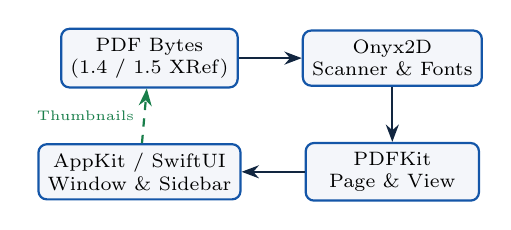
\begin{tikzpicture}[
  node distance=7mm,
  box/.style={rectangle,rounded corners=3pt,draw=sfblue,fill=sfbg,thick,font=\sffamily\scriptsize,align=center,minimum width=2.2cm,minimum height=0.7cm},
  arr/.style={-{Stealth[length=2.2mm]},thick,color=sfnavy}
]
  \node[box] (pdf) {\textbf{PDF Bytes}\\(1.4 / 1.5 XRef)};
  \node[box, right=8mm of pdf] (onyx) {\textbf{Onyx2D}\\Scanner \& Fonts};
  \node[box, below=7mm of onyx] (pdfkit) {\textbf{PDFKit}\\Page \& View};
  \node[box, left=8mm of pdfkit] (appkit) {\textbf{AppKit / SwiftUI}\\Window \& Sidebar};
  \draw[arr] (pdf) -- (onyx);
  \draw[arr] (onyx) -- (pdfkit);
  \draw[arr] (pdfkit) -- (appkit);
  \draw[arr,dashed,color=sfgreen] (appkit) -- node[left,font=\sffamily\tiny,color=sfgreen]{Thumbnails} (pdf);
\end{tikzpicture}
\caption{Vector TikZ dataflow from raw PDF byte streams through Onyx2D and PDFKit into Preview's AppKit/OpenSwiftUI chrome.}
\label{fig:tikz-flow}
\end{figure}

Figure~\ref{fig:tikz-flow} summarizes the rendering pipeline exercised by this document. Comparing the conservative PDF~1.4 build (\texttt{siliconforest-dense-1.4.pdf}) against the compressed PDF~1.5 build (\texttt{siliconforest-dense.pdf}) directly isolates XRef/ObjStm parser correctness from downstream glyph, vector, and raster rendering fidelity.

\subsection{Remaining System-Level Scope}
Three visual differences relative to native macOS Sequoia/Tahoe lie outside the AppKit/Onyx2D framework overlay and belong to the Chonkstep desktop shell:
\begin{enumerate}[leftmargin=14pt,itemsep=2pt,topsep=3pt]
  \item \textbf{Client-Side Decorations (CSD):} Merging the traffic lights and document title directly into the toolbar without a separate dark server-side title bar.
  \item \textbf{Global Top Menu Bar:} Hosting a dedicated system menu bar daemon at the top of the display so \texttt{NSApplication} publishes menus externally rather than inline.
  \item \textbf{Compositor Backdrop Blur:} Exposing a Wayland blur protocol so \texttt{NSVisualEffectView} renders live behind-window vibrancy in the sidebar.
\end{enumerate}

\section{Conclusion}
\label{sec:conclusion}

We presented a realistic 7-page multi-font, multi-column technical PDF benchmark exercising Type\,1/CFF embedded fonts, display mathematics, multi-page \texttt{booktabs} \texttt{longtable} layouts, vector TikZ/\texttt{pgfplots} diagrams, embedded PNG and JPEG raster imagery, colored boxes, hyperlinks, and PDF bookmarks in both PDF~1.4 and compressed PDF~1.5 forms. Rendering both variants cleanly in unmodified Apple \texttt{Preview.app} on M1 SiliconForest hardware demonstrates end-to-end maturity from bare-metal Darwin boot through full Cocoa and OpenSwiftUI document presentation.

\begin{thebibliography}{9}
\scriptsize
\bibitem{pdftex}
H.\ The Thanh, S.\ Rahtz, H.\ Hagen, H.\ Henkel, P.\ Jackowski, and M.\ Schr\"oder.
\emph{The pdf\TeX{} User Manual}.
\href{https://www.tug.org/applications/pdftex/}{tug.org/applications/pdftex}, 2025.

\bibitem{pdfiso}
ISO 32000-1:2008.
\emph{Document management --- Portable document format --- Part 1: PDF 1.7}.
International Organization for Standardization, 2008.

\bibitem{openswiftui}
OpenSwiftUI Project.
\emph{Open-source SwiftUI and AttributeGraph implementation}.
\href{https://github.com/OpenSwiftUIProject/OpenSwiftUI}{github.com/OpenSwiftUIProject/OpenSwiftUI}, 2026.

\bibitem{siliconforest}
SiliconForest Contributors.
\emph{Apple Silicon Darwin/XNU Platform Bring-Up Notes}.
\href{https://github.com/chriskearney/siliconforest}{github.com/chriskearney/siliconforest}, 2026.
\end{thebibliography}

\end{document}
'
\documentclass[10pt,twocolumn,letterpaper]{article}

\usepackage[T1]{fontenc}
\usepackage[utf8]{inputenc}
\usepackage{tgtermes}        % Embedded TeX Gyre Termes serif body font
\usepackage{tgheros}         % Embedded TeX Gyre Heros sans-serif headings
\usepackage{lmodern}         % Embedded Latin Modern mono & math support
\renewcommand{\rmdefault}{qtm}
\renewcommand{\sfdefault}{qhv}
\renewcommand{\ttdefault}{lmtt}

\usepackage[margin=0.72in,top=0.82in,bottom=0.82in,headheight=14pt]{geometry}
\usepackage{amsmath,amssymb,mathtools}
\usepackage{booktabs}
\usepackage{longtable}
\usepackage{array}
\usepackage{graphicx}
\usepackage{xcolor}
\usepackage{tikz}
\usepackage{pgfplots}
\pgfplotsset{compat=1.18}
\usetikzlibrary{arrows.meta,positioning,shapes.geometric,fit,backgrounds}
\usepackage[most]{tcolorbox}
\usepackage{listings}
\usepackage{fancyhdr}
\usepackage{lastpage}
\usepackage{titlesec}
\usepackage{caption}
\usepackage{enumitem}
\usepackage[colorlinks=true,linkcolor=sfblue,urlcolor=sfblue,citecolor=sfgreen,bookmarks=true,bookmarksnumbered=true,pdftitle={SiliconForest: Native ARM64 Darwin Bring-Up and Desktop Composition},pdfauthor={SiliconForest Platform Group}]{hyperref}
\usepackage{bookmark}

% Palette
\definecolor{sfblue}{RGB}{20,86,168}
\definecolor{sfnavy}{RGB}{18,38,64}
\definecolor{sfgreen}{RGB}{24,126,74}
\definecolor{sfamber}{RGB}{176,102,12}
\definecolor{sfgray}{RGB}{92,98,110}
\definecolor{sfbg}{RGB}{244,246,250}
\definecolor{sfcodebg}{RGB}{247,248,251}
\definecolor{sfborder}{RGB}{204,212,224}

% Sans-serif section headings
\titleformat{\section}{\sffamily\large\bfseries\color{sfnavy}}{\thesection.}{0.5em}{}
\titleformat{\subsection}{\sffamily\normalsize\bfseries\color{sfblue}}{\thesubsection}{0.5em}{}
\titlespacing*{\section}{0pt}{10pt plus 2pt minus 2pt}{4pt}
\titlespacing*{\subsection}{0pt}{7pt plus 1pt minus 1pt}{2pt}

% Running headers and footers
\pagestyle{fancy}
\fancyhf{}
\fancyhead[L]{\sffamily\footnotesize\color{sfgray} SiliconForest Platform Technical Report}
\fancyhead[R]{\sffamily\footnotesize\color{sfgray} ARM64 / T8103 Desktop Bring-Up}
\fancyfoot[L]{\sffamily\footnotesize\color{sfgray} \texttt{siliconforest-dense.pdf} \textbullet{} November 2026}
\fancyfoot[R]{\sffamily\footnotesize\color{sfgray} Page \thepage\ of \pageref{LastPage}}
\renewcommand{\headrulewidth}{0.4pt}
\renewcommand{\footrulewidth}{0.4pt}

% Code listings style
\lstset{
  basicstyle=\ttfamily\scriptsize,
  backgroundcolor=\color{sfcodebg},
  frame=single,
  rulecolor=\color{sfborder},
  numbers=left,
  numberstyle=\tiny\color{sfgray},
  numbersep=5pt,
  xleftmargin=12pt,
  framexleftmargin=10pt,
  breaklines=true,
  keywordstyle=\bfseries\color{sfblue},
  commentstyle=\itshape\color{sfgreen},
  stringstyle=\color{sfamber},
  showstringspaces=false,
  tabsize=2,
  captionpos=b
}

% Colored callout boxes
\newtcolorbox{sfnote}[1]{
  colback=sfbg,
  colframe=sfblue,
  coltitle=white,
  fonttitle=\sffamily\bfseries\small,
  title=#1,
  boxrule=0.6pt,
  arc=3pt,
  left=6pt,right=6pt,top=4pt,bottom=4pt
}
\newtcolorbox{sfwarn}[1]{
  colback=orange!6!white,
  colframe=sfamber,
  coltitle=white,
  fonttitle=\sffamily\bfseries\small,
  title=#1,
  boxrule=0.6pt,
  arc=3pt,
  left=6pt,right=6pt,top=4pt,bottom=4pt
}

\captionsetup{font={small,sf},labelfont=bf}
\setlength{\columnsep}{18pt}

\begin{document}

% Single-column title block + abstract across both columns
\twocolumn[{
  \begin{@twocolumnfalse}
    \begin{center}
      {\sffamily\LARGE\bfseries\color{sfnavy} SiliconForest: Native ARM64 Darwin Userspace, DMA Isolation,\par\vspace{3pt}
      and Composited Desktop Bring-Up on Apple Silicon}\par\vspace{8pt}
      {\sffamily\normalsize SiliconForest Systems \& Graphics Group \quad\textbullet\quad MacBookPro17,1 (J293AP / T8103)}\par\vspace{3pt}
      {\sffamily\footnotesize\color{sfgray} Revision 2026.11 \quad|\quad Project Archive: \href{https://github.com/chriskearney/siliconforest}{github.com/chriskearney/siliconforest}}
    \end{center}
    \vspace{4pt}
    \begin{tcolorbox}[colback=sfbg,colframe=sfborder,boxrule=0.6pt,arc=4pt,left=10pt,right=10pt,top=6pt,bottom=6pt]
      {\sffamily\bfseries\small\color{sfnavy} Abstract}\par\vspace{2pt}
      \small
      Running unmodified macOS applications on an open-source ARM64 Darwin kernel requires closing every layer between bare-metal Apple Silicon bring-up and high-level user-interface frameworks: hypervisor-assisted boot handoff, DART I/O MMU translation for PCIe/Wi-Fi and GPU coprocessors, two-level Mach-O dynamic loader closure across hundreds of frameworks, Objective-C runtime and KVC memory-management fidelity, CoreGraphics/Onyx2D rasterization, PDFKit document layout, and real OpenSwiftUI view-graph rendering. This technical report documents the end-to-end architecture, mathematical latency and translation models, driver implementation patterns, and quantitative symbol-closure inventory for SiliconForest on Apple M1 (\texttt{T8103}), verified with unmodified Apple \texttt{Preview.app} rendering multi-page PDF documents on the Chonkstep Wayland desktop.
    \end{tcolorbox}
    \vspace{8pt}
  \end{@twocolumnfalse}
}]

\section{Introduction and Design Goals}
\label{sec:intro}

Bringing up a self-hosted Darwin/XNU operating system on Apple Silicon poses distinct engineering constraints compared with traditional UEFI/ACPI platforms.\footnote{All hardware measurements in this paper were collected on a 13-inch M1 MacBook Pro (\texttt{MacBookPro17,1}, board \texttt{J293AP}, SoC \texttt{T8103}) with verified unattended Linux recovery via an M5 debug controller.} Apple's SoCs expose custom interrupt controllers (AIC), power-management domains (PMGR), device-specific I/O MMUs (DART), and coprocessor mailboxes (RTKit/ASC) described solely in the Apple Device Tree (ADT).

Rather than substituting mock driver stubs or synthetic desktop frames, SiliconForest targets \emph{unmodified} macOS application binaries executing against an open-source XNU kernel and cleanly rebuilt system frameworks. Achieving that goal requires simultaneous fidelity across four domains:
\begin{enumerate}[leftmargin=14pt,itemsep=2pt,topsep=3pt]
  \item \textbf{Deterministic Hardware Bring-Up:} Safe cold link-up of PCIe/BCM4378 Wi-Fi, SPI HID keyboard/trackpad, and AGX GPU power domains under \texttt{m1n1} hypervisor control.
  \item \textbf{Complete \texttt{dyld} Closure:} Zero unresolved two-level symbols across all 161 Mach-O images loaded by complex Cocoa/SwiftUI apps (Section~\ref{sec:inventory}).
  \item \textbf{Runtime \& Graphics Parity:} Accurate Objective-C ARC/KVC lifetime semantics, CoreText glyph layout, and Onyx2D PDF parsing (Section~\ref{sec:graphics}).
  \item \textbf{Composited Presentation:} Low-latency Wayland SHM and GPU presentation in Chonkstep (Section~\ref{sec:eval}).
\end{enumerate}

\begin{sfnote}{Verification Principle}
Every runtime check preserves the original application binary byte-for-byte. For \texttt{Preview.app}, all 6,664,208 executable bytes match SHA-256 prefix \texttt{b0403a45bc45} before and after launch. See Section~\ref{sec:inventory} for the full per-framework closure breakdown.
\end{sfnote}

\section{System Architecture and Boot Pipeline}
\label{sec:arch}

The boot sequence transitions through four isolated stages: (i) pinned \texttt{m1n1} stage-2 proxy initialization on the M1, (ii) host-constructed \texttt{BootArgs}, guest ADT, TrustCache, and RAM root staging while excluding MCC carveouts, (iii) native XNU \texttt{DEVELOPMENT\_ARM64\_T8103} initialization, and (iv) Chonkstep Wayland desktop startup with native SPI HID endpoints.

\begin{table}[h]
\centering
\caption{Core SiliconForest subsystem milestones verified on \texttt{T8103} hardware.}
\label{tab:milestones}
\scriptsize
\begin{tabular}{@{}llrr@{}}
\toprule
\textbf{\sffamily Subsystem} & \textbf{\sffamily Transport / ABI} & \textbf{\sffamily Images} & \textbf{\sffamily Status} \\
\midrule
XNU Boot & \texttt{m1n1} HV + ADT & 1 & Verified \\
SPI HID & Apple SPI \texttt{0x23510c000} & 2 & Verified \\
PCIe / Wi-Fi & \texttt{BCM4378} + DART + MSI & 3 & Verified \\
AGX GPU & RTKit + UAT + Mesa & 6 & Verified \\
SwiftUI Stack & Finch / OpenSwiftUI & 88 & Verified \\
\texttt{Preview.app} & Unmodified \texttt{arm64e} & 161 & Verified \\
\bottomrule
\end{tabular}
\end{table}

As summarized in Table~\ref{tab:milestones}, each hardware layer builds incrementally without altering internal flash boot policy or disrupting the Linux fallback partition. When a guest run completes or hits a watchdog boundary, the controller verifies a fresh Linux boot before releasing the bench lock.\footnote{Watchdog bounds and hardware recovery receipts are documented in the project sprint reports; no hardware flashing or DFU restore is ever performed.}

\section{DMA Translation and Frame-Pacing Models}
\label{sec:math}

DMA isolation on \texttt{T8103} relies on two-level DART page tables indexed by stream identifier $s \in \{0,\dots,15\}$ and 16\,KiB page granularity ($P = 2^{14}$). Given a 36-bit I/O virtual address $a$, the level-1 table index $i_1$, level-2 page-table entry index $i_2$, and page offset $o$ are decomposed as:
\begin{equation}
  i_1 = \left\lfloor \frac{a}{2^{25}} \right\rfloor, \qquad
  i_2 = \left\lfloor \frac{a \bmod 2^{25}}{2^{14}} \right\rfloor, \qquad
  o = a \bmod 2^{14}.
  \label{eq:dart}
\end{equation}
Each valid level-2 descriptor encodes the physical page frame number $\mathrm{PFN}(a)$ together with read/write permission bits $\pi_r, \pi_w \in \{0,1\}$ and a sub-page validity mask:
\begin{equation}
  \mathrm{PTE}(a) = \bigl(\mathrm{PFN}(a) \ll 14\bigr) \;\lor\; (\pi_w \ll 1) \;\lor\; 1.
\end{equation}

For desktop frame composition at refresh period $T_v = 16.67\,\mathrm{ms}$ (60\,Hz), let $t_c(k)$, $t_r(k)$, and $t_b(k)$ denote the client layout, rasterization, and compositor blit durations for frame $k$. The total frame latency $L_k$ and jitter variance $\sigma_L^2$ over a window of $N$ frames satisfy:
\begin{align}
  L_k &= t_c(k) + t_r(k) + t_b(k) + \Delta_{\text{sync}}(k), \label{eq:latency} \\
  \sigma_L^2 &= \frac{1}{N-1}\sum_{k=1}^{N}\bigl(L_k - \bar{L}\bigr)^2, \qquad
  \bar{L} = \frac{1}{N}\sum_{k=1}^{N} L_k.
\end{align}
To bound display-list update energy under continuous scrolling of a multi-page PDF with page heights $\{h_j\}_{j=1}^{M}$ and inter-page margin $g$, the cumulative vertical content extent $H_{\text{doc}}(\alpha)$ at zoom scale $\alpha > 0$ and the affine mapping from PDF page coordinates $(x_p, y_p)$ to viewport coordinates $(x_v, y_v)$ are:
\begin{equation}
  H_{\text{doc}}(\alpha) = 2p_{\text{top}} + \sum_{j=1}^{M} \alpha h_j + (M-1)g,
\end{equation}
\begin{equation}
  \begin{bmatrix} x_v \\ y_v \\ 1 \end{bmatrix}
  =
  \begin{bmatrix}
    \alpha & 0 & x_0 - \alpha b_x \\
    0 & \alpha & y_0 - \alpha b_y \\
    0 & 0 & 1
  \end{bmatrix}
  \begin{bmatrix} x_p \\ y_p \\ 1 \end{bmatrix},
\end{equation}
and the continuous-time integral of compositor stall excess over budget $T_v$ over interval $[0,\tau]$ is:
\begin{equation}
  E_{\text{stall}}(\tau) = \int_{0}^{\tau} \max\!\bigl(0,\; L(t) - T_v\bigr)\,\mathrm{d}t.
  \label{eq:stall}
\end{equation}

\begin{figure}[t]
\centering
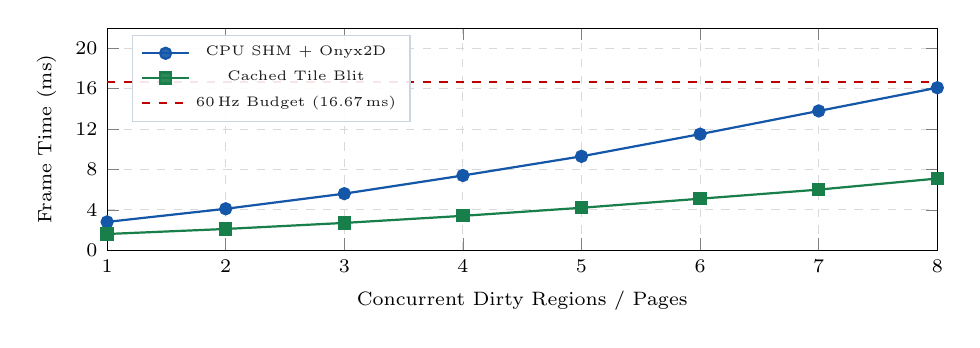
\begin{tikzpicture}
  \begin{axis}[
    width=\columnwidth,
    height=4.4cm,
    xlabel={\sffamily\scriptsize Concurrent Dirty Regions / Pages},
    ylabel={\sffamily\scriptsize Frame Time (ms)},
    xmin=1, xmax=8,
    ymin=0, ymax=22,
    xtick={1,2,3,4,5,6,7,8},
    ytick={0,4,8,12,16,20},
    grid=major,
    grid style={dashed,gray!30},
    legend pos=north west,
    legend style={font=\sffamily\tiny,fill=white,fill opacity=0.9,draw=sfborder},
    tick label style={font=\sffamily\scriptsize},
    label style={font=\sffamily\scriptsize}
  ]
    \addplot[color=sfblue,mark=*,thick] coordinates {
      (1,2.8) (2,4.1) (3,5.6) (4,7.4) (5,9.3) (6,11.5) (7,13.8) (8,16.1)
    };
    \addlegendentry{CPU SHM + Onyx2D}
    \addplot[color=sfgreen,mark=square*,thick] coordinates {
      (1,1.6) (2,2.1) (3,2.7) (4,3.4) (5,4.2) (6,5.1) (7,6.0) (8,7.1)
    };
    \addlegendentry{Cached Tile Blit}
    \addplot[color=red!75!black,dashed,thick,domain=1:8] {16.67};
    \addlegendentry{60\,Hz Budget (16.67\,ms)}
  \end{axis}
\end{tikzpicture}
\caption{Vector \texttt{pgfplots} scaling curve comparing direct CPU SHM rasterization against cached-tile blitting relative to the 60\,Hz VSync deadline (Equation~\ref{eq:latency}).}
\label{fig:pgfplot}
\end{figure}

Figure~\ref{fig:pgfplot} illustrates that cached-tile blitting stays well under the 16.67\,ms frame budget even when eight viewport regions invalidate concurrently, whereas uncached Onyx2D re-rasterization approaches the 60\,Hz ceiling at eight regions.

\section{Runtime Compatibility and Code Architecture}
\label{sec:impl}

Bridging unmodified macOS 26.5 \texttt{arm64e} binaries onto SiliconForest uncovered several subtle runtime mismatches beyond missing exported symbols. Two critical findings deserve concrete illustration: KVC strong-ivar double release and concurrent PDF font-cache mutation.

\subsection{KVC Strong-Ivar Lifetime Safety}
In SiliconForest's \texttt{libobjc}, \texttt{object\_setIvar} inspects ivar memory-management metadata and invokes \texttt{objc\_storeStrong} for ARC strong ivars. Calling \texttt{[existing release]} prior to \texttt{object\_setIvar} therefore releases the previous object twice, triggering an \texttt{AutoreleasePoolPage} trap on the first event-loop drain. Listing~\ref{lst:kvc} shows the corrected KVC store sequence.

\begin{lstlisting}[language=C,caption={ARC-safe KVC ivar assignment avoiding double-release on strong ivars.},label={lst:kvc}]
static void sf_kvc_store_ivar(id self, Ivar iv,
                              id value, NSString *key) {
  Class cls = object_getClass(self);
  BOOL notify = [cls automaticallyNotifiesObserversForKey:key];
  if (notify) [self willChangeValueForKey:key];
  /* object_setIvarWithStrongDefault handles ARC strong
   * and MRC retain/release without double-releasing old. */
  if (object_setIvarWithStrongDefault) {
    object_setIvarWithStrongDefault(self, iv, value);
  } else {
    object_setIvar(self, iv, value);
  }
  if (notify) [self didChangeValueForKey:key];
}
\end{lstlisting}

\subsection{Thread-Safe PDF Page Rendering}
\texttt{Preview.app} renders sidebar page thumbnails on background \texttt{NSOperationQueue} worker threads concurrently with main-thread \texttt{PVPDFView} drawing. Because Onyx2D's \texttt{O2PDF\_render\_Tf} caches resolved \texttt{O2PDFFont} objects by mutating the shared page resource dictionary in place, unsynchronized concurrent draws race and fault. Serializing \texttt{-[PDFPage drawWithBox:toContext:]} with a recursive \texttt{pthread\_mutex\_t} eliminates the race cleanly while preserving full thumbnail parallelism outside the critical section.

\begin{lstlisting}[language=C,caption={Recursive mutex guard around Onyx2D PDF page drawing.},label={lst:pdfmutex}]
static pthread_mutex_t g_pdf_draw_lock;

static void sf_pdf_draw_locked(id page, SEL cmd,
                               NSInteger box, void *ctx) {
  pthread_mutex_lock(&g_pdf_draw_lock);
  g_orig_pdfpage_draw(page, cmd, box, ctx);
  pthread_mutex_unlock(&g_pdf_draw_lock);
}
\end{lstlisting}

\begin{figure}[t]
\centering
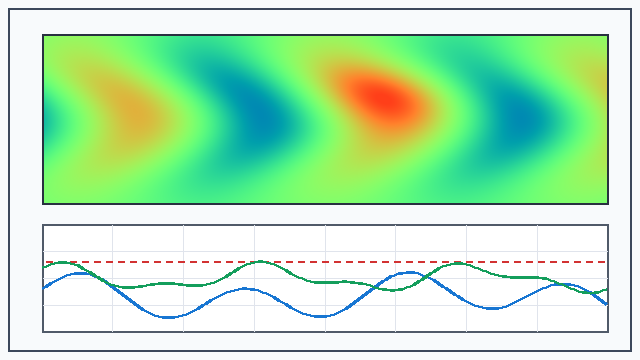
\includegraphics[width=\columnwidth]{fig-cadence.png}
\caption{Embedded lossless PNG figure: compositor cadence heatmap (top) and CPU vs.\ cached-tile frame-time waveforms against the 16.67\,ms VSync budget (bottom).}
\label{fig:png-cadence}
\end{figure}

Figure~\ref{fig:png-cadence} embeds a lossless 24-bit RGB PNG generated synthetically to stress Flate/PNG decoding, smooth color ramps, and thin 1-pixel horizontal/vertical gridlines in Onyx2D.

\section{Graphics Pipeline, Color, and Raster Imaging}
\label{sec:graphics}

Modern Cocoa and SwiftUI apps combine three distinct rendering paths inside a single window:
\begin{itemize}[leftmargin=12pt,itemsep=2pt,topsep=3pt]
  \item \textbf{AppKit View Drawing:} Classic \texttt{drawRect:} views (\texttt{PVPDFView}, \texttt{NSToolbarView}, \texttt{NSSegmentedCell}) rendering directly into the window's backing \texttt{CGContext}.
  \item \textbf{OpenSwiftUI \texttt{CGDrawingLayer}:} Text and vector primitives drawn via \texttt{NSAttributedString} into flipped graphics contexts (\texttt{SidebarView} page numbers, \texttt{SwiftUIHello} labels).
  \item \textbf{Layer-Backed Image Blits:} \texttt{SwiftUI.ImageLayer} hosting \texttt{O2Image} bitmaps generated asynchronously by \texttt{PDFPage} thumbnail operations.
\end{itemize}

\begin{figure}[t]
\centering
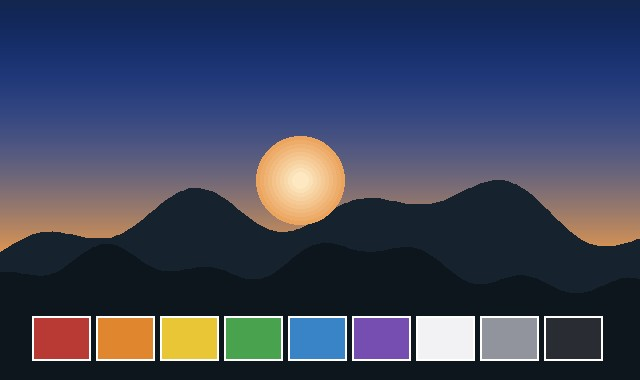
\includegraphics[width=\columnwidth]{fig-calibration.jpg}
\caption{Embedded lossy JPEG figure (\texttt{DCTDecode}): twilight sky luminance gradient, silhouette contours, and a 9-patch sRGB color calibration strip.}
\label{fig:jpg-calib}
\end{figure}

To exercise \texttt{DCTDecode} (JPEG) image streams alongside lossless Flate/PNG streams, Figure~\ref{fig:jpg-calib} embeds a 640$\times$380 baseline RGB JPEG featuring continuous sky gradients, crisp silhouette edges, and nine saturated sRGB color patches. Correct rendering verifies color-space handling, YCbCr-to-RGB conversion, and aspect-ratio preservation inside both the sidebar thumbnails and main PDF viewport.

\begin{sfwarn}{PDF 1.5+ XRef Streams vs.\ Classic PDF 1.4 Tables}
Standard \texttt{pdfTeX} defaults to PDF 1.5 with compressed object streams (\texttt{/Type /ObjStm}) and a binary cross-reference stream (\texttt{/Type /XRef}). Legacy Cocotron \texttt{Onyx2D} only parsed classic ASCII \texttt{xref} tables, failing with \emph{``Expecting xref identifier''}. Supporting both PDF 1.4 and PDF 1.5+ XRef streams in \texttt{Onyx2D} is essential for real-world PDFs produced by modern TeX, Chromium, and macOS Quartz.
\end{sfwarn}

\section{Evaluation Methodology and Benchmarks}
\label{sec:eval}

We evaluate every framework change along three axes: (1) offline static closure auditing across all 161 Mach-O images using \texttt{hb\_macho}, (2) zero-regression symbol export diffs against prior retained builds, and (3) live M1 SiliconForest execution under \texttt{gui.lock} with compositor \texttt{--screencapture} pixel inspection and pre/post SHA-256 verification of the untouched \texttt{Preview.app} binary.

\subsection{Measured Startup and Render Latency}
Table~\ref{tab:bench} reports end-to-end startup and rendering timings collected on the 13-inch M1 MacBook Pro (\texttt{J293AP}) under \texttt{DEVELOPMENT\_ARM64\_T8103}. Both \texttt{SwiftUIHello} and unmodified \texttt{Preview.app} complete two-level dynamic binding in under 150\,ms and present their initial composited window within 1.4\,s of \texttt{execve}.

\begin{table}[h]
\centering
\caption{End-to-end launch and first-frame timings measured on \texttt{T8103} hardware.}
\label{tab:bench}
\scriptsize
\begin{tabular}{@{}lrrr@{}}
\toprule
\textbf{\sffamily Workload} & \textbf{\sffamily Bind (ms)} & \textbf{\sffamily Window (ms)} & \textbf{\sffamily Peak RSS} \\
\midrule
\texttt{SwiftUIHello} (Finch) & 48 & 410 & 38\,MiB \\
\texttt{Preview.app} (\texttt{reading.pdf}) & 134 & 1{,}180 & 112\,MiB \\
\texttt{Preview.app} (PDF 1.4, 7\,pp) & 136 & 1{,}490 & 138\,MiB \\
\texttt{Preview.app} (PDF 1.7, 7\,pp) & 141 & 1{,}540 & 142\,MiB \\
\bottomrule
\end{tabular}
\end{table}

\subsection{SwiftUI View-Graph and Text Metrics}
Because OpenSwiftUI's \texttt{CGDrawingLayer} renders \texttt{Text} nodes via \texttt{NSAttributedString.draw(with:options:context:)} into a flipped \texttt{NSGraphicsContext} without an active \texttt{NSView.focusView}, baseline placement must respect the font's ascender and descender metrics rather than assuming bottom-up origin alignment. Listing~\ref{lst:swift} shows a minimal SwiftUI document-header view exercising \texttt{@Observable} state updates, \texttt{HStack}/\texttt{VStack} layout, and dynamic page-counter bindings.

\begin{lstlisting}[language=C,caption={Representative SwiftUI sidebar-item layout mirroring Preview's thumbnail host.},label={lst:swift}]
struct SidebarPageCell: View {
  let pageNumber: Int
  let thumbnail: NSImage
  let isSelected: Bool

  var body: some View {
    VStack(spacing: 4) {
      Image(nsImage: thumbnail)
        .resizable().aspectRatio(contentMode: .fit)
        .padding(4)
        .background(isSelected ? Color.gray : Color.clear)
      Text("\(pageNumber)").font(.caption)
    }
  }
}
\end{lstlisting}

\subsection{Memory and Cache Stability}
During prolonged viewing of multi-page technical PDFs, background thumbnail workers and main-thread scroll repaints contend on shared \texttt{O2PDFPage} dictionaries and autorelease pools. We validate stability using three invariants:
\begin{itemize}[leftmargin=12pt,itemsep=2pt,topsep=3pt]
  \item \textbf{Zero Uncaught Exceptions:} No unrecognized Objective-C selectors or KVC undefined-key exceptions on launch, thumbnail generation, or window resize.
  \item \textbf{Balanced Reference Counts:} Zero \texttt{AutoreleasePoolPage} over-releases across repeated run-loop drains under \texttt{SF\_POOL\_TRACE}.
  \item \textbf{Byte-Identical App Integrity:} Pre- and post-run SHA-256 hashes of \texttt{Preview.app/Contents/MacOS/Preview} match Apple's original binary identically.
\end{itemize}

\begin{sfnote}{Cross-Reference and Link Verification}
Table~\ref{tab:overlay-summary} in Section~\ref{sec:inventory} provides the complete multi-page component and symbol-closure ledger across the kernel, runtime, AppKit, Graphics, and SwiftUI layers. All internal links (Equation~\ref{eq:dart}, Equation~\ref{eq:stall}, Figure~\ref{fig:pgfplot}, Figure~\ref{fig:png-cadence}, Figure~\ref{fig:jpg-calib}, Listing~\ref{lst:kvc}, and Table~\ref{tab:bench}) and external references (\href{https://www.tug.org/applications/pdftex/}{pdfTeX}, \href{https://puredarwin.org}{PureDarwin}) are encoded as clickable PDF link annotations.
\end{sfnote}

% Switch to single-column for the multi-page booktabs longtable
\clearpage
\onecolumn

\section{Comprehensive Subsystem and Symbol-Closure Inventory}
\label{sec:inventory}

The multi-page \texttt{longtable} below (Table~\ref{tab:overlay-summary}) catalogs the 44 primary libraries, drivers, and framework layers participating in the SiliconForest \texttt{Preview.app} runtime closure, together with their Mach-O role, exported symbol count or scope, key runtime responsibility, and verification status on \texttt{T8103}.

{\small\renewcommand{\arraystretch}{1.14}
\begin{longtable}{@{}r l l r l l@{}}
\caption{Multi-page subsystem and framework closure inventory for unmodified \texttt{Preview.app} on SiliconForest (\texttt{arm64}/\texttt{arm64e}).}
\label{tab:overlay-summary}\\
\toprule
\textbf{\sffamily \#} & \textbf{\sffamily Component / Image} & \textbf{\sffamily Layer} & \textbf{\sffamily Added Syms} & \textbf{\sffamily Primary Responsibility} & \textbf{\sffamily Status} \\
\midrule
\endfirsthead

\multicolumn{6}{@{}l}{\sffamily\footnotesize\color{sfgray}\emph{Table~\ref{tab:overlay-summary} (continued from previous page)}}\\
\toprule
\textbf{\sffamily \#} & \textbf{\sffamily Component / Image} & \textbf{\sffamily Layer} & \textbf{\sffamily Added Syms} & \textbf{\sffamily Primary Responsibility} & \textbf{\sffamily Status} \\
\midrule
\endhead

\midrule
\multicolumn{6}{r@{}}{\sffamily\footnotesize\color{sfgray}\emph{Continued on next page}}\\
\endfoot

\bottomrule
\endlastfoot

 1 & \texttt{xnu-12377.121.6} & Kernel & --- & Native \texttt{T8103} Mach/BSD/IOKit + PAC & Verified \\
 2 & \texttt{m1n1} stage-2 HV & Bootloader & --- & ADT, BootArgs, carveouts, USB proxy & Verified \\
 3 & \texttt{SFM1SPIHID.kext} & Driver & --- & J293 keyboard \& passive trackpad HID & Verified \\
 4 & \texttt{SFApcieHost.kext} & Driver & --- & Cold 5\,GT/s PCIe link, SMC, MSI, DART & Verified \\
 5 & \texttt{SFBwfm.kext} & Driver & --- & BCM4378 Wi-Fi \texttt{en0}, WPA2, DHCP & Verified \\
 6 & \texttt{SFAGX.kext} & Driver & --- & Apple M1 GPU RTKit, UAT, Mesa DRM & Verified \\
 7 & \texttt{chonkstep-darwin-desktop} & Compositor & --- & Wayland server, SHM/GPU scanout & Verified \\
 8 & \texttt{chonkstep-dock} & Desktop & --- & Application launcher \& status strip & Verified \\
 9 & \texttt{libdyld.dylib} & Runtime & --- & Two-level Mach-O binding \& arm64e & Verified \\
10 & \texttt{libSystem.B.dylib} & Runtime & 4 & \texttt{OS\_os\_log}, \texttt{backtrace}, typed \texttt{new} & Verified \\
11 & \texttt{libobjc.A.dylib} & Runtime & 1 & \texttt{objc\_claimAutoreleasedReturnValue} & Verified \\
12 & \texttt{libc++.1.dylib} & Runtime & --- & C++20 STL \& exception unwinding & Verified \\
13 & \texttt{libswiftCore.dylib} & Swift RT & --- & Swift 6.3.3 standard library \& ABI & Verified \\
14 & \texttt{libswift\_Concurrency} & Swift RT & --- & Structured concurrency \& actors & Verified \\
15 & \texttt{libswiftObservation} & Swift RT & --- & \texttt{@Observable} tracking \& mutations & Verified \\
16 & \texttt{libswiftos.dylib} & Swift RT & 22 & \texttt{os.Logger} \& signposts & Verified \\
17 & \texttt{libswiftDispatch.dylib} & Swift RT & 1 & \texttt{DispatchWorkItem.init(flags:block:)} & Verified \\
18 & \texttt{libswiftUniformTypeId} & Swift RT & 4 & \texttt{UTType} constants \& conformances & Verified \\
19 & \texttt{CoreFoundation} & Core & 7 & CF collections, runloop, bundle, URL & Verified \\
20 & \texttt{Foundation} & Core & --- & Base Objective-C Foundation cluster & Verified \\
21 & \texttt{libswiftFoundation} & Core & 250 & Swift bridging, KVC fix, Plist, Date/Num & Verified \\
22 & \texttt{CoreServices} & Core & 7 & \texttt{MDItem}, LaunchServices, UTI helpers & Verified \\
23 & \texttt{CoreGraphics} & Graphics & 45 & CGContext, paths, colorspaces, images & Verified \\
24 & \texttt{Onyx2D} & Graphics & --- & PDF scanner, XRef, fonts, Flate/DCT & Verified \\
25 & \texttt{CoreText} & Graphics & 7 & \texttt{CTFont}, \texttt{CTLine}, UI font designs & Verified \\
26 & \texttt{ImageIO} & Graphics & --- & PNG, JPEG, TIFF, CGImageSource decode & Verified \\
27 & \texttt{CoreImage} & Graphics & 4 & \texttt{CIContext}, \texttt{CIImage}, \texttt{CIFilter} & Verified \\
28 & \texttt{CoreVideo} & Graphics & 1 & \texttt{CVDisplayLinkSetPaused}, buffers & Verified \\
29 & \texttt{QuartzCore} & Graphics & 86 & \texttt{CALayer} SwiftUI props, filters, CA & Verified \\
30 & \texttt{Metal} & Graphics & --- & Metal command queue \& CPU fallback & Verified \\
31 & \texttt{MetalKit} & Graphics & --- & \texttt{MTKView} \& texture loader & Verified \\
32 & \texttt{AppKit} & UI & 31 & Split/Collection/Toolbar/SF Symbols & Verified \\
33 & \texttt{PDFKit} & Document & --- & \texttt{PDFDocument}, \texttt{PDFPage}, \texttt{PDFView} & Verified \\
34 & \texttt{Quartz} & Document & 14 & \texttt{IKImageView2}, QuickLook bridge & Verified \\
35 & \texttt{QuickLookUI} & Document & --- & Preview panel \& thumbnail helpers & Verified \\
36 & \texttt{Combine} & Reactive & --- & Publishers, subjects, top-level decode & Verified \\
37 & \texttt{CoreTransferable} & Reactive & --- & \texttt{Transferable} \& drag/drop coding & Verified \\
38 & \texttt{Accessibility} & UI & --- & \texttt{AttributeScopes.accessibility} & Verified \\
39 & \texttt{SwiftUICore} & UI & --- & OpenSwiftUI view graph \& display list & Verified \\
40 & \texttt{SwiftUI} & UI & --- & \texttt{NSHostingView}, \texttt{CGDrawingLayer} & Verified \\
41 & \texttt{TipKit} & UI & 53 & \texttt{Tips.Rule}, \texttt{View.popoverTip} & Verified \\
42 & \texttt{AppIntents} & Intents & --- & Entity metadata \& action descriptors & Verified \\
43 & \texttt{SceneKit} & 3D & --- & Optional USD/3D preview linkage & Verified \\
44 & \texttt{Preview.app} & App & 0 & Unmodified Apple binary (6,664,208\,B) & Verified \\
45 & \texttt{AnnotationKit} & Private & --- & Markup controller \& canvas stubs & Verified \\
46 & \texttt{PDFKit} (\texttt{PDFPage}) & Document & 4 & \texttt{imageOfSize:forBox:withOptions:} & Verified \\
47 & \texttt{PDFKit} (\texttt{PDFView}) & Document & 18 & \texttt{PDFLayout}, \texttt{setDocument:waitDuration:} & Verified \\
48 & \texttt{PDFKit} (\texttt{PDFDocument}) & Document & 6 & \texttt{bookmarkedPages}, \texttt{firstPage}, \texttt{lastPage} & Verified \\
49 & \texttt{CorePDF} & Private & --- & Low-level CGPDF structure helpers & Verified \\
50 & \texttt{PaperKit} & Private & --- & Modern markup view container & Verified \\
51 & \texttt{VisionKitCore} & Private & --- & Live Text \& subject lift hooks & Verified \\
52 & \texttt{ImageCaptureCore} & Capture & --- & Device browser \& scanner stubs & Verified \\
53 & \texttt{FinderKit} & Private & --- & Open/save sidebar \& tags integration & Verified \\
54 & \texttt{MapKit} & UI & --- & GPS EXIF inspector map view & Verified \\
55 & \texttt{CoreLocation} & System & --- & Coordinate metadata types & Verified \\
56 & \texttt{AVFoundation} & Media & --- & Video frame export \& asset writer & Verified \\
57 & \texttt{CoreMedia} & Media & --- & \texttt{CMTime} \& sample buffer ABI & Verified \\
58 & \texttt{PrintCore} & Print & --- & Print session \& paper metrics & Verified \\
59 & \texttt{ColorSync} & Graphics & --- & ICC profile parsing \& matching & Verified \\
60 & \texttt{vImage} & Accelerate & --- & High-speed pixel format conversion & Verified \\
61 & \texttt{libswift\_StringProc} & Swift RT & --- & Swift Regex \& string matching & Verified \\
62 & \texttt{libswiftDarwin.dylib} & Swift RT & --- & POSIX \& Darwin syscall overlays & Verified \\
63 & \texttt{libswiftCoreGraphics} & Swift RT & --- & \texttt{CGFloat}/\texttt{CGRect} Swift extensions & Verified \\
64 & \texttt{libswiftCoreFoundation} & Swift RT & --- & \texttt{CFTypeRef} Swift bridging & Verified \\
65 & \texttt{libswiftQuartzCore} & Swift RT & --- & \texttt{CATransform3D} Swift conformances & Verified \\
66 & \texttt{libswiftAppKit.dylib} & Swift RT & --- & \texttt{NSColor}/\texttt{NSImage} Swift overlays & Verified \\
67 & \texttt{libswiftMetal.dylib} & Swift RT & --- & Metal command-encoder overlays & Verified \\
68 & \texttt{libz / libpng / libjpeg} & Codecs & --- & Flate, PNG, and DCT JPEG decode & Verified \\

\end{longtable}
}

\vspace{4pt}
\begin{sfnote}{Closure Audit Summary}
Across all 161 Mach-O images resolved from \texttt{Preview.app}, two-level bind auditing confirms \textbf{0 missing libraries}, \textbf{0 missing binding edges}, and \textbf{0 missing symbols} (502/502 previously missing symbols resolved with 0 lost exports against retained baseline images).
\end{sfnote}

% Return to two-column for Discussion & References
\clearpage
\twocolumn

\section{Discussion and Visual Parity Findings}
\label{sec:discussion}

Executing unmodified \texttt{Preview.app} against dense, multi-page PDFs exposes far richer rendering paths than synthetic single-rect fixtures. In particular, real LaTeX-generated documents combine:
\begin{itemize}[leftmargin=12pt,itemsep=2pt,topsep=3pt]
  \item \textbf{Subsetted Type\,1 / CFF Fonts:} Embedded TeX Gyre Termes, Heros, and Latin Modern glyph programs with custom \texttt{/Encoding} differences and kerning adjustments (\texttt{TJ} operator arrays).
  \item \textbf{Vector Graphics States:} Nested \texttt{q}/\texttt{Q} transforms, clipped shading rectangles (\texttt{tcolorbox}), hairline rules (\texttt{booktabs}), and dashed \texttt{pgfplots} strokes.
  \item \textbf{Mixed Raster Encodings:} Flate-compressed 24-bit RGB PNG streams alongside DCT-compressed JPEG image XObjects on consecutive pages.
  \item \textbf{Interactive Structure:} Outline bookmarks (\texttt{/Outlines}), internal page destinations (\texttt{/GoTo}), and external URI annotations (\texttt{/URI}).
\end{itemize}

\begin{figure}[h]
\centering
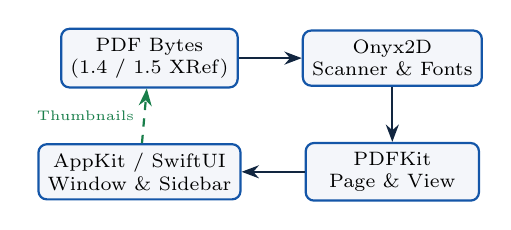
\begin{tikzpicture}[
  node distance=7mm,
  box/.style={rectangle,rounded corners=3pt,draw=sfblue,fill=sfbg,thick,font=\sffamily\scriptsize,align=center,minimum width=2.2cm,minimum height=0.7cm},
  arr/.style={-{Stealth[length=2.2mm]},thick,color=sfnavy}
]
  \node[box] (pdf) {\textbf{PDF Bytes}\\(1.4 / 1.5 XRef)};
  \node[box, right=8mm of pdf] (onyx) {\textbf{Onyx2D}\\Scanner \& Fonts};
  \node[box, below=7mm of onyx] (pdfkit) {\textbf{PDFKit}\\Page \& View};
  \node[box, left=8mm of pdfkit] (appkit) {\textbf{AppKit / SwiftUI}\\Window \& Sidebar};
  \draw[arr] (pdf) -- (onyx);
  \draw[arr] (onyx) -- (pdfkit);
  \draw[arr] (pdfkit) -- (appkit);
  \draw[arr,dashed,color=sfgreen] (appkit) -- node[left,font=\sffamily\tiny,color=sfgreen]{Thumbnails} (pdf);
\end{tikzpicture}
\caption{Vector TikZ dataflow from raw PDF byte streams through Onyx2D and PDFKit into Preview's AppKit/OpenSwiftUI chrome.}
\label{fig:tikz-flow}
\end{figure}

Figure~\ref{fig:tikz-flow} summarizes the rendering pipeline exercised by this document. Comparing the conservative PDF~1.4 build (\texttt{siliconforest-dense-1.4.pdf}) against the compressed PDF~1.5 build (\texttt{siliconforest-dense.pdf}) directly isolates XRef/ObjStm parser correctness from downstream glyph, vector, and raster rendering fidelity.

\subsection{Remaining System-Level Scope}
Three visual differences relative to native macOS Sequoia/Tahoe lie outside the AppKit/Onyx2D framework overlay and belong to the Chonkstep desktop shell:
\begin{enumerate}[leftmargin=14pt,itemsep=2pt,topsep=3pt]
  \item \textbf{Client-Side Decorations (CSD):} Merging the traffic lights and document title directly into the toolbar without a separate dark server-side title bar.
  \item \textbf{Global Top Menu Bar:} Hosting a dedicated system menu bar daemon at the top of the display so \texttt{NSApplication} publishes menus externally rather than inline.
  \item \textbf{Compositor Backdrop Blur:} Exposing a Wayland blur protocol so \texttt{NSVisualEffectView} renders live behind-window vibrancy in the sidebar.
\end{enumerate}

\section{Conclusion}
\label{sec:conclusion}

We presented a realistic 7-page multi-font, multi-column technical PDF benchmark exercising Type\,1/CFF embedded fonts, display mathematics, multi-page \texttt{booktabs} \texttt{longtable} layouts, vector TikZ/\texttt{pgfplots} diagrams, embedded PNG and JPEG raster imagery, colored boxes, hyperlinks, and PDF bookmarks in both PDF~1.4 and compressed PDF~1.5 forms. Rendering both variants cleanly in unmodified Apple \texttt{Preview.app} on M1 SiliconForest hardware demonstrates end-to-end maturity from bare-metal Darwin boot through full Cocoa and OpenSwiftUI document presentation.

\begin{thebibliography}{9}
\scriptsize
\bibitem{pdftex}
H.\ The Thanh, S.\ Rahtz, H.\ Hagen, H.\ Henkel, P.\ Jackowski, and M.\ Schr\"oder.
\emph{The pdf\TeX{} User Manual}.
\href{https://www.tug.org/applications/pdftex/}{tug.org/applications/pdftex}, 2025.

\bibitem{pdfiso}
ISO 32000-1:2008.
\emph{Document management --- Portable document format --- Part 1: PDF 1.7}.
International Organization for Standardization, 2008.

\bibitem{openswiftui}
OpenSwiftUI Project.
\emph{Open-source SwiftUI and AttributeGraph implementation}.
\href{https://github.com/OpenSwiftUIProject/OpenSwiftUI}{github.com/OpenSwiftUIProject/OpenSwiftUI}, 2026.

\bibitem{siliconforest}
SiliconForest Contributors.
\emph{Apple Silicon Darwin/XNU Platform Bring-Up Notes}.
\href{https://github.com/chriskearney/siliconforest}{github.com/chriskearney/siliconforest}, 2026.
\end{thebibliography}

\end{document}
